\documentclass[11pt]{article}

% Links
\usepackage{hyperref}
\makeatletter
\g@addto@macro{\UrlBreaks}{\UrlOrds}
\makeatother

% Margins
\usepackage[left=20mm, bottom=30mm,right=20mm]{geometry}

% Maths
\usepackage{siunitx}
\usepackage{amsmath}

% Code
\usepackage{float}
\usepackage{listings}
\definecolor{codegreen}{rgb}{0,0.6,0}
\definecolor{codegray}{rgb}{0.5,0.5,0.5}
\definecolor{codepurple}{rgb}{0.58,0,0.82}
\definecolor{backcolour}{rgb}{0.95,0.95,0.92}
\lstdefinestyle{mystyle}{
    backgroundcolor=\color{backcolour},   
    commentstyle=\color{codegreen},
    keywordstyle=\color{magenta},
    numberstyle=\tiny\color{codegray},
    stringstyle=\color{codepurple},
    basicstyle=\ttfamily\footnotesize,
    breakatwhitespace=false,         
    breaklines=true,                 
    captionpos=b,                    
    keepspaces=true,                 
    numbers=left,                    
    numbersep=5pt,                  
    showspaces=false,                
    showstringspaces=false,
    showtabs=false,                  
    tabsize=2
}
\lstset{style=mystyle}


% Underlines
\usepackage{ulem}

% Imports
\usepackage{import}

% Graphics
\usepackage{graphicx}

% Plots
\usepackage{pgfplots}
\pgfplotsset{width=10cm,compat=1.9}

% Picture for title
\usepackage[demo]{graphicx}
\usepackage{subcaption}
\usepackage{titlepic}

% Language 
% \usepackage[english]{babel}

% Headers and footers
\usepackage{fancyhdr}
\pagestyle{fancyplain}
\fancyhf{}
\lhead{\fancyplain{}{Redes de Computadores - 1º Trabalho Laboratorial}}
\lfoot{\fancyplain{}{}}
\cfoot{\thepage}

% Paragraph indentation
\usepackage{indentfirst}

% Picture
\titlepic{\begin{figure}[t!]
\centering
\subfloat{{
\includegraphics[width=7cm]{img/unnamed.png} }}%
\qquad
\subfloat{{
\includegraphics[width=7cm]{img/Cienciasporto.png} }}%
%\vspace{-3.0cm}
\end{figure}}
% Date
\date{Janeiro, 2022}
% Title
\title{\textbf{\Huge{Applicação de Download FTP e Laboratórios de Configuração de Rede} \\ \\ \\
\Large{  Licenciatura em Engenharia Informática e Computação \newline Redes de Computadores - 2º Trabalho Laboratorial }}}
% Author
\author{
\textbf{\Large Class 9 group 2} \vspace{0.5em} \\
\begin{tabular}{r l}
	\email{up201906086@edu.fe.up.pt} & Marcelo Henriques Couto \\
	\email{up201907361@edu.fe.up.pt} & Francisco Pinto de Oliveira \\
\end{tabular}
}

% No paragraph indentation
% \parindent=0pt

% Start the document
\begin{document}
\maketitle

\newpage
\tableofcontents

\newpage
\input{Sumário}
\section{Sumário}

Este relatório tem pretende descrever a implementação do 1º trabalho laboratorial de Redes de Computadores, expondo detalhes de funcionamento, implementação e eficiência.

O trabalho foi concluído com sucesso e a aplicação é capaz de transmitir ficheiros utilizando a porta série.


\section{Introdução}

O trabalho desenvolvido teve como objetivo desenvolver um protocolo de transmissão de dados através da porta série. Este relatório pretende descrever o funcionamento e detalhes de implementação.

O relatório será organizado nos seguintes módulos:
\begin{itemize}
    \item \textbf{Arquitetura} – blocos funcionais e interfaces
    \item \textbf{Estrutura do código} – principais funções e estruturas de dados bem como a sua relação com a arquitetura
    \item \textbf{Casos de uso} – identificação e sequencia de chamada de funções
    \item \textbf{Protocolo de ligação lógica} – descrição de funcionamento do protocolo e exemplificação apresentando fragmentos de código
    \item \textbf{Protocolo da aplicação} – descrição do funcionamento da camada e exemplificação apresentando fragmento de código
    \item \textbf{Validação} – descrição dos testes efetuados
    \item \textbf{Eficiência do protocolo de ligação de dados} – caracterização da eficiência do protocolo de ligação de dados
    \item \textbf{Conclusões} – síntese da informação apresentada nas secções anteriores e reflexão sobre objetivos e aprendizagens
\end{itemize}
    
\newpage
\section{Aplicação FTP}

\subsection{Arquitetura da aplicação}

A primeira parte do projeto desenvolvido insidia em criar uma aplicação capaz de executar transferências através de um URL utilizando o protocolo FTP (File Transfer Protocol). No desenvolvimento da aplicação foram tidas em conta as normas \href{https://www.rfc-editor.org/info/rfc959}{RFC959} \href{https://www.rfc-editor.org/info/rfc1738}{RFC1738}, respeitantes à comunicação com o servidor e interpretação do URL respetivamente.

\subsubsection{Interpretação do URL}
A primeira parte da aplicação está responsável por interpretar os argumentos contidos no URL, bem como verificar a sua validade. A função \textbf{create\_url\_data-url\_path\_parser.c}:

\begin{enumerate}
    \item Verifica se o URL corresponde a um protocolo FTP utilizando a função \textbf{is\_ftp}
    \item Interpreta o utilizador e a password presentes (ou não) no URL, que estarão localizadas logo a seguir ao protocolo e separados por ':' e com '@' a marcar o seu fim
    \item Deteta a eventual presença de uma porta com recurso à função \textbf{has\_port} e, em caso positivo, guarda o seu valor
    \item Analiza o caminho e servidor presentes, separa-os, guarda o caminho e o endereço IP com recurso à função \textbf{gethostbyname - netdb.h}
\end{enumerate}

Todos os dados interpretados do URL são guardados numa struct do tipo \textbf{URLPathData}.

\subsubsection{Execução da transferência}
Depois de interpretados os dados do URL necessários para a execução da transferência é necessário comunicar o servidor e efetuar o download do ficheiro pretendido. A função \textbf{ftp\_download - ftp.c}:

\begin{enumerate}
    \item \textbf{ftp\_control\_connect:} Estabelece uma ligação ao servidor (socket) no modo de controlo à porta 21, com recurso à função \textbf{connect - sys/socket.h}
    \item \textbf{ftp\_login:} Efetua autenticação no servidor com as credenciais obtidas pelo URL (comandos USER e PASS e respetivos argumentos são enviados pelo socket)
    \item \textbf{ftp\_retrieve\_passive\_mode:} Envia um pedido de conexão em modo passivo (comando PASV) \textbf{*}
    \item \textbf{ftp\_data\_connect:} Estabelece uma ligação de dados à porta recebida pelo servidor como resposta ao pedido anterior 
    \item \textbf{ftp\_change\_dir\_to\_res:} Na conexão de controlo, muda de diretório para o diretório correto e envia o comando RETR para iniciar o download
    \item \textbf{f\_retrieve\_fd:} Cria um cicheiro local com o mesmo nome do ficheiro remoto
    \item \textbf{ftp\_dump\_data:} Realiza a transferência do ficheiro
    \item \textbf{ftp\_close:} Fecha as conexões com o servidor
\end{enumerate}

Cada pedido ao servidor retorna uma mensagem, da qual retiramos o código através da função \textbf{ftp\_read\_resp\_code}. Este código é interpretado de modo a entender se o procedimento está a seguir o seu curso esperado ou se, a algum momento, houve um erro ou rejeição por parte do servidor.

\textbf{*} em modo passivo, o comando enviado ao servidor é \textbf{PASV} em vez de \textbf{PORT}, sendo o servidor a retornar a porta por onde a ligação de dados deve ser estabelecida e a transferência efetuada

\subsection{Exemplo de Download e Resultados}

A aplicação foi testada com ficheiros de diferentes tamanhos, tipos e de diferentes fontes, sendo experimentado ambos o modo anónimo (sem credenciais) e com autenticação no servidor. Abaixo temos alguns exemplos de execução documentados.

\begin{figure}[!h]
\centering
  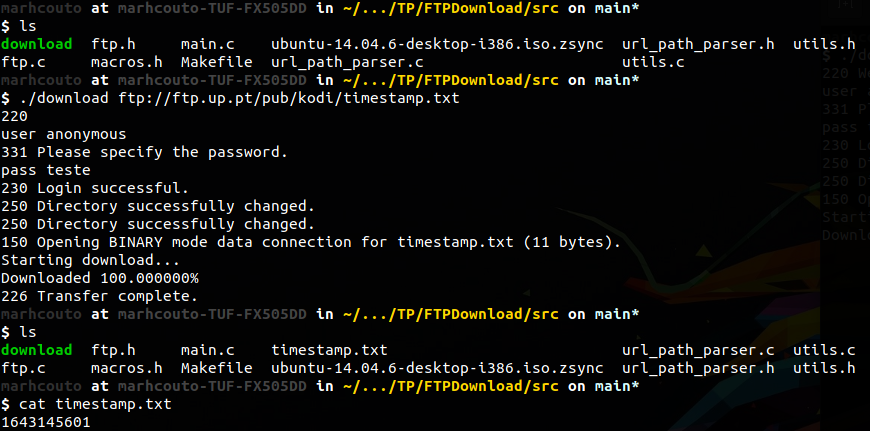
\includegraphics[width=.6\linewidth]{img/Download1.png}
  \caption{Transferência de ficheiro timestamp - 11B}
\end{figure}

\begin{figure}[!h]
\centering
  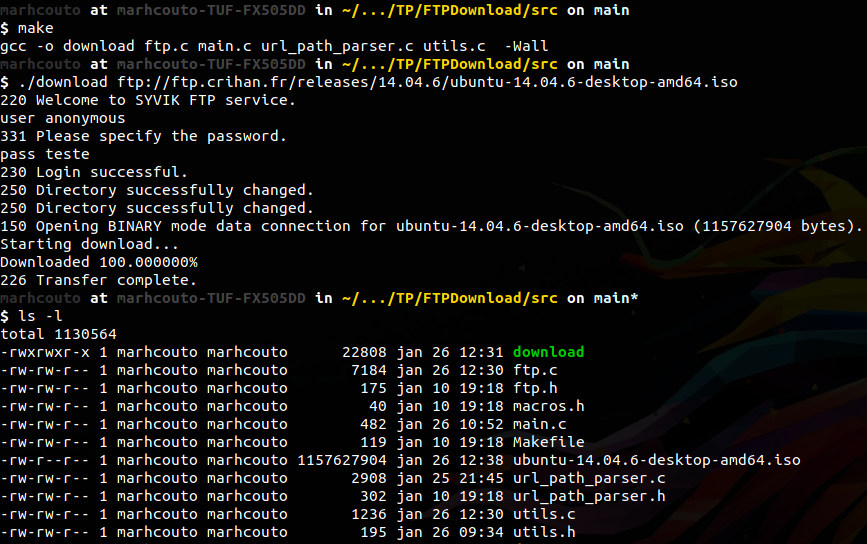
\includegraphics[width=.6\linewidth]{img/Download2.png}
  \caption{Ubuntu iso - 1104 MB}
\end{figure}

\newpage
\section{Configuração de uma Rede}

\subsection{Experiência 1}

Nesta experiência configuraram-se endereços IP de duas máquinas ligadas através de um switch para entender melhor como funciona a comuniação entre máquinas e o significado e funcionamento de pacotes ARP.

\begin{figure}[!h]
\centering
  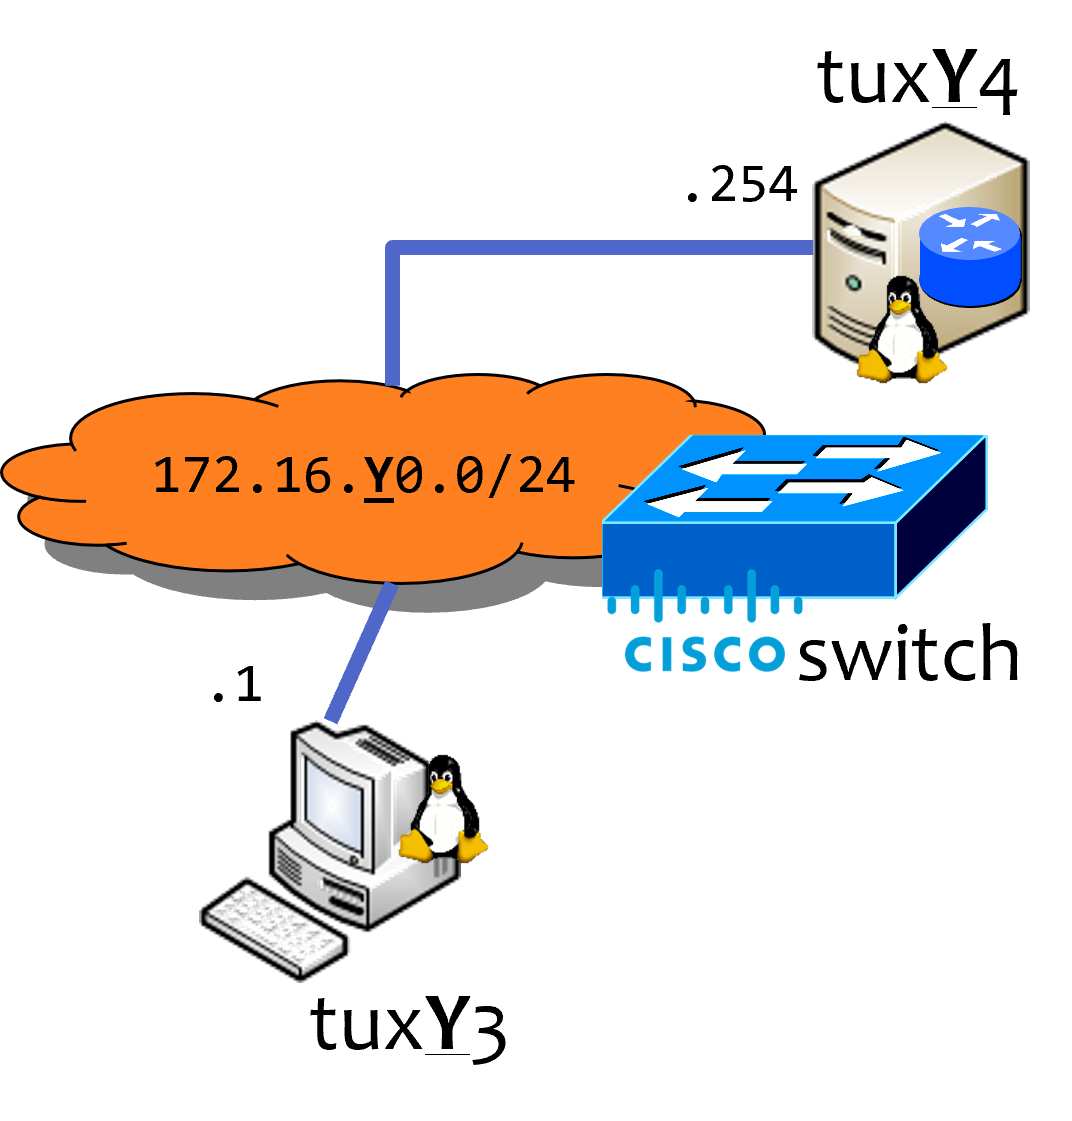
\includegraphics[width=.3\linewidth]{img/exp1-net.png}
  \caption{Estrutura da rede}
\end{figure}

\subsubsection{Questões}

\paragraph{O que são os pacotes ARP e para que são usados?}
Os pacotes do protocolo ARP são utilizados para, sabendo o endereço IP de uma maquina, descobrir o seu endereço MAC. 

\paragraph{O que são os endereços MAC e IP dos pacotes ARP e porquê?}
Os endereços MAC identificam as interfaces com a rede que uma determinada máquina utiliza para comunicar com outras máquinas. Nos pacotes ARP utilizados para pedir o endereço MAC da interface de uma máquina, o primeiro endereço é enviado para que se identifique o endereço IP da máquina cujo endereço MAC é procurado. O segundo é utilizado para identificar a máquina que pretende ser informada. Nos pacotes ARP de resposta, o primeiro endereço IP é enviado para identificar a máquina que possui o endereço MAC enviado em segundo lugar.

\paragraph{Que pacotes gera o comando PING?}
São gerados pacotes ICMP utilizados para mandar erros da camada 3 ou mensagens para routers. Neste caso são utilizados para testar a conectividade entre as máquinas da rede.

\paragraph{Quais são os endereços IP e MAC dos pacotes de PING?}
O endereço IP de origem dos pacotes enviados é 172.16.50.1, o endereço do tux53. O endereço IP de destino é 172.16.50.254, o endereço de IP do tux54.  O endereço MAC de origem dos pacotes é 00:21:5a:61:2d:72 o endereço de eth0 do tux53. O endereço MAC de destino é 00:21:5a:c3:78:70, o endereço de eth0 do tux54. 

\paragraph{Como determinar se um frame Ethernet recebido é ARP, IP, ICMP?}
Ao analisar os pacotes no Wireshark pode verificar-se o tipo de frame analisando os bytes 12-13 do pacote recebido. Os pacotes ARP têm tipo 0x0806 os pacotes IP têm tipo 0x0800. Os pacotes ICMP têm o mesmo tipo dos pacotes IP e o byte 23 é 0x01. O Wireshark faz esta análise portanto basta ver a coluna Protocol para cada pacote.

\paragraph{Como determinar o comprimento da trama recebida?}
O comprimento das tramas pode ser observado no Wireshark na coluna Length. As tramas IP possuem o seu tamanho nos bytes 16-17.


\subsection{Experiência 2}

Esta experiência teve como objetivo configurar duas VLAN's, bem como entender como funcionam domínios de broadcast.

\begin{figure}[!h]
\centering
  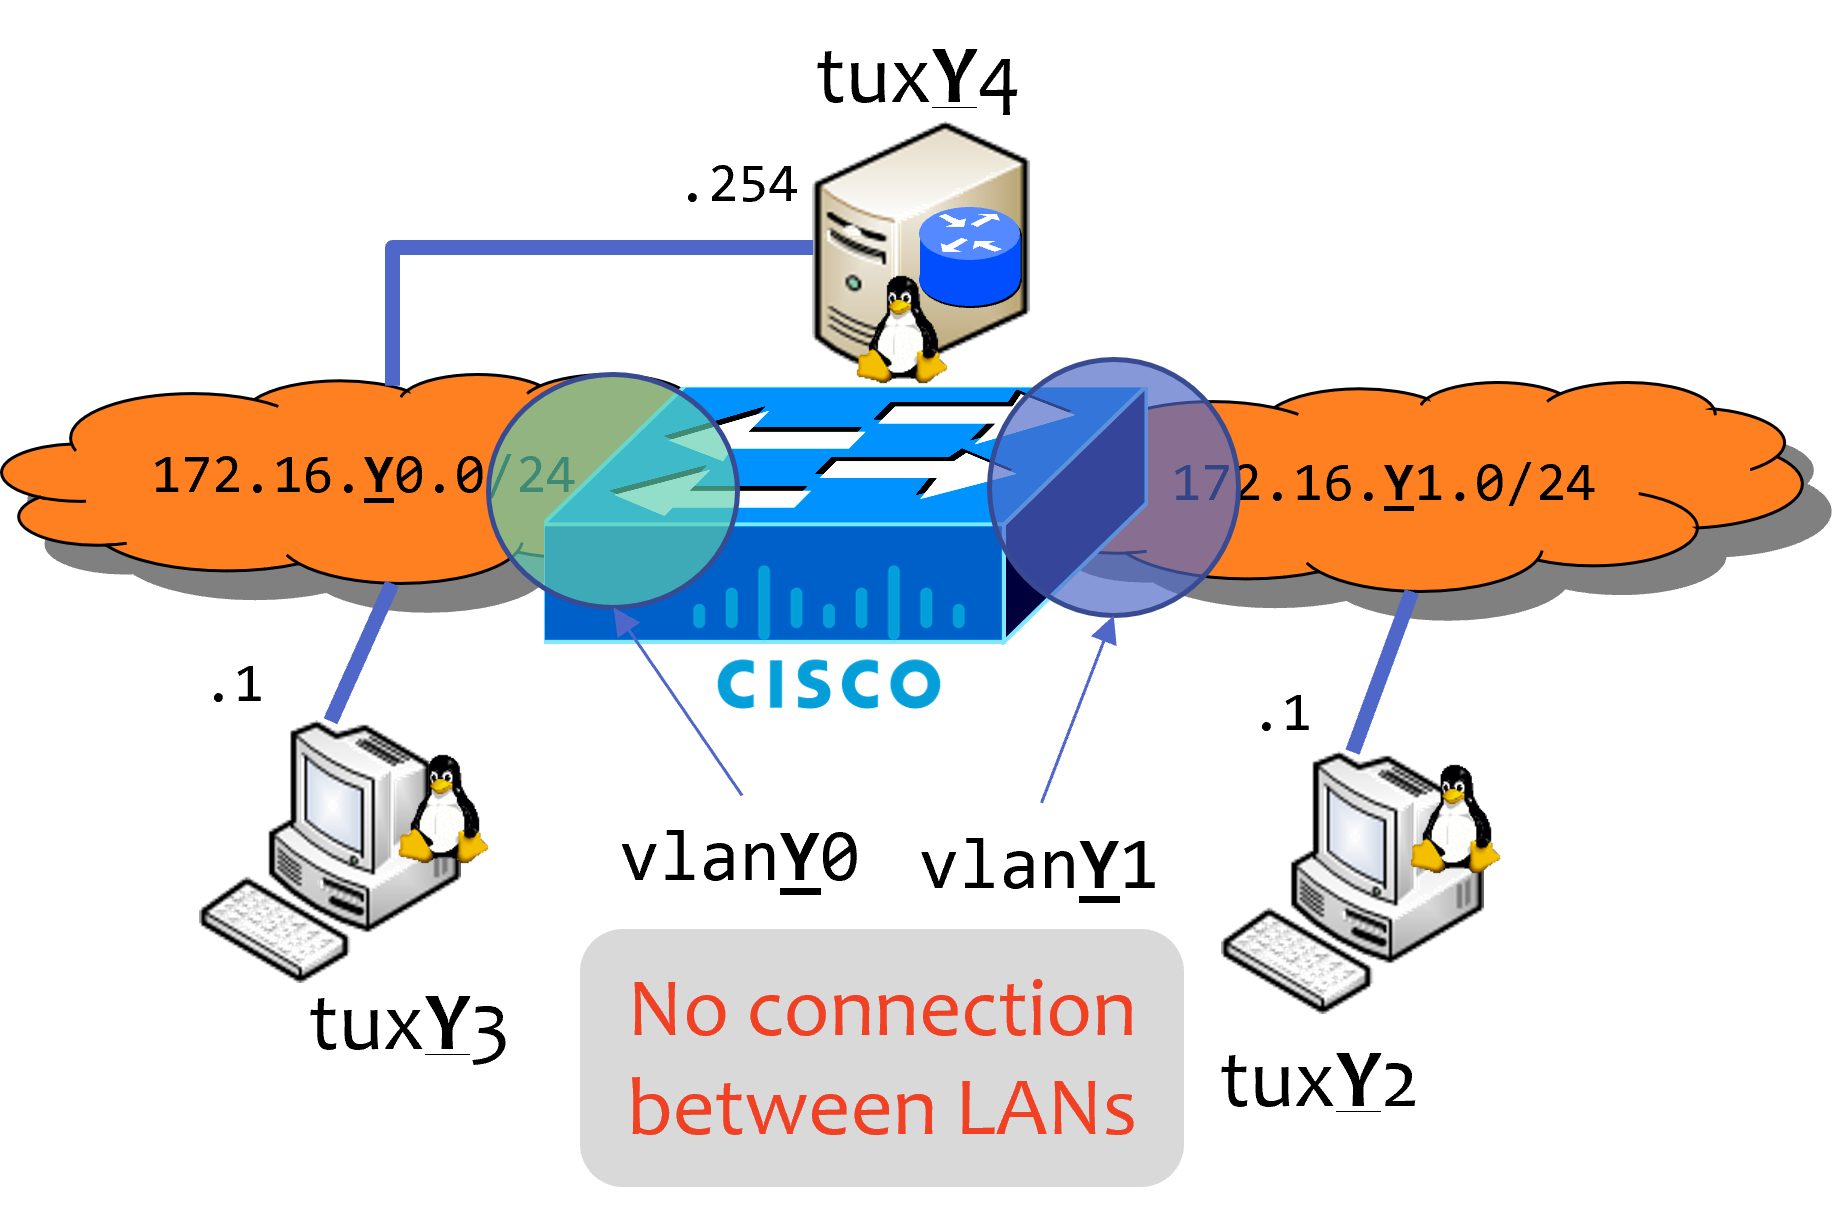
\includegraphics[width=.4\linewidth]{img/net-vlans.png}
  \caption{Estrutura da rede}
\end{figure}

\subsubsection{Questões}
\paragraph{Como configurar a vlan50}
Primeiro conecta-se a interface eht0 do tux53 à conexão correspondente à porta 1 do switch e o a interface eth0 do tux54 à conexão correspondente à porta 2. Em seguida configuramos os endereços IP de ambas as interfaces para que correspondam à especificação


\begin{center}
\begin{tabular}{ c c c }
    \textbf{Máquina} & \textbf{Interface} & \textbf{Endereço IP} \\ \hline 
    Tux53 & eth0 & 172.16.50.1 \\  
    Tux54 & eth0 & 172.16.50.254    
\end{tabular}
\end{center}


Em seguida criamos conectamos a porta série do Tux53 à porta série do switch e configuramos a VLAN50 com as portas 1 e 2 associadas à VLAN pois são as portas a que estão conectados os Tux53 e Tux54.

\paragraph{Quantos dominios de broadcast há? Como o podemos cocluir tendo por base os logs?}

Podemos concluir que há dois domínios de Broadcast. Um deles é na vlan50, uma vez que, os pacotes do ping do tux3 (172.16.50.1) atingem o tux4 (172.16.50.254), mas não atingem tux2(172.16.51.1) como se pode ver nas figuras (Figure 10 e Figure 12). O outro é na vlan51, no entanto, não há qualquer prova de Broadcast porque o tux2 se encontra isolado na vlan referida havendo apenas registo dos pacotes a saírem da origem como se pode ver na figura. (Figure 14)
\subsection{Experiência 3}

Esta experiência possibilitou o entendimento do sistema de DNS bem como a configuração de NAT num router comercial.

\begin{figure}[!h]
\centering
  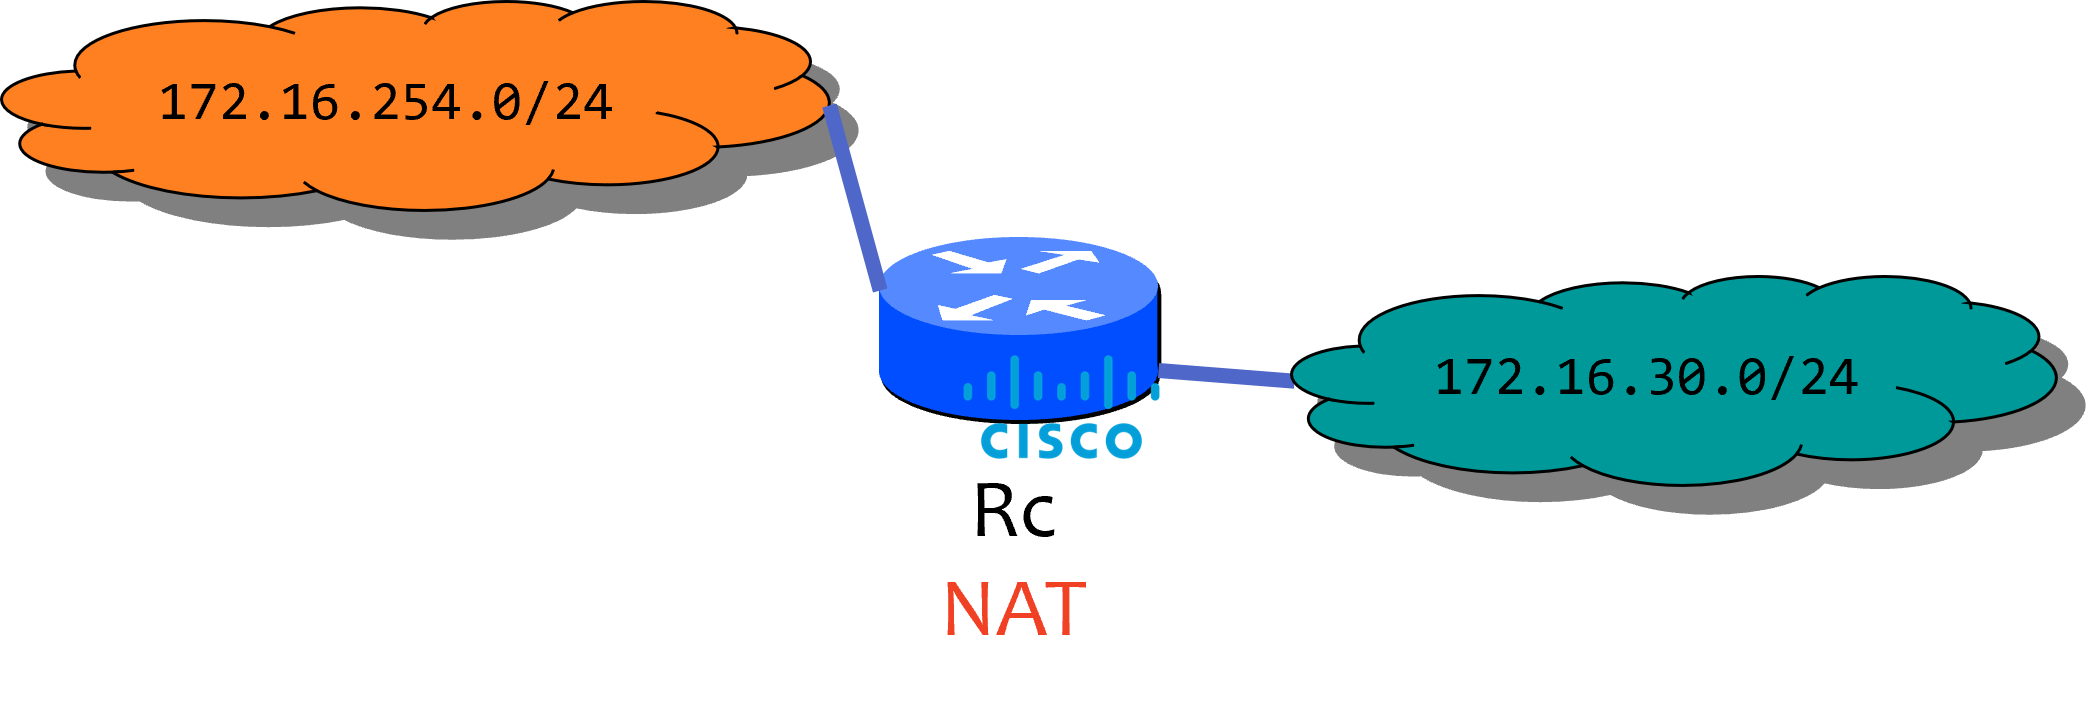
\includegraphics[width=.4\linewidth]{img/net-routing-nat-cisco.png}
  \caption{Estrutura da rede}
\end{figure}

\subsubsection{Questões}

\paragraph{Como configurar uma rota estática num router comercial?}

Executando o seguinte comando:  
    \begin{center} \lstinline{ip route 172.16.40.0 255.255.255.0 172.16.30.2} \end{center}

O primeiro endereço refere-se ao prefixo de origem dos pacotes, o segundo endereço é a máscara de sub-rede, e o último endereço é o gateway dos pacotes.

\paragraph{Como configurar NAT num router comercial?}
Para configurar a NAT deve-se seguir os seguintes comandos:
 - Identificar a interface de rede com o comando: interface FastEthernet0/0
 - Atribuir o endereço de IP que a interface vai tomar nessa NAT com: ip address 172.16.30.1 255.255.255.0
 - Especificar o tipo de NAT interno ou externo (neste caso externo): ip nat inside

Após configurar a interface deve configurar-se a pool de endereços exteriores disponiveis com: ip nat pool ovrld 172.16.254.45 172.16.254.45 prefix-length 24

Por fim, basta configurar a pool IP's internos:
\begin{itemize}
    \item ip nat inside source list 1 pool ovrld overload
    \item access-list 1 permit 172.16.40.0 0.0.0.7
    \item access-list 1 permit 172.16.30.0 0.0.0.7
\end{itemize}


\paragraph{O que faz a NAT?}
NAT é uma técnica que permite mapear uma gama de endereços IP para outra gama de endereços IP mudando o IP dos pacotes enviados enquanto estão em trânsito. É utilizada geralmente para mapear o endereço IP público fornecido por um ISP para o endereço privado da máquina do utilizador.

\paragraph{Como configurar o serviço de DNS no host?}
Pode-se configurar traduções especificas em /etc/hosts como fizemos com o mapeamento do endereço de youtubas. Pode-se configurar um servidor central que faz a tradução no ficheiro /etc/resolv.conf adicionando: nameserver {IP_DNS}

\paragraph{Que pacotes são trocados pelo DNS e que informação é transportada}
São observados dois tipos de pacote muito semelhantes. Ambos transportam o hostname sobre o qual se quer saber o IP. A resposta aos pacotes do tipo 'A' é um endereço IPv4, já a resposta ao pacotes AAAA é um endereço IPv6.

\paragraph{Que pacotes ICMP são observados e porquê?}
O traceroute tenta encontrar o número mínimo de saltos para alcançar um determinado destino. Para isso gera pacotes UDP com TTL crescente partindo de 1. Quando recebe um pacote ICPM que informa que TTL foi excedido o traceroute sabe que necessita de pelo menos mais um valor de TTL para alcançar o destino. No nosso caso como o destino não aceita pedidos é ainda enviado um pacote ICPM que informa que a porta é inalcançável.

\paragraph{Quais são os endereços IP e MAC associados a pacotes ICMP e porquê?}
Os endereços IP de destino são sempre da nossa máquina, os de origem correspondem aos vários IP intermédios pelos quais os pacotes devem viajar até alcançar o destino (Figure 18). Cada vez que o traceroute aumenta o TTL, o endereço de origem muda, o que significa que o pacote atingiu mais um nó. O endereço MAC de origem é sempre o endereço MAC da interface virtual do computador host, o o endereço de destino é o MAC da interface virtual do Guest OS.

\paragraph{Quais são as rotas na sua máquina? Qual o seu significado?}
A rota com origem em 0.0.0.0 e  destino em 172.24.64.1 é a default gateway é indica por onde devem ser enviados os pacotes caso não possam ser encaminhados para a rede local. (Figure 19)

A rota com origem em 172.24.64.0 e gateway 0.0.0.0 é a rota inválida para pacotes com destino inválido.
\subsection{Experiência 4}

Esta experiência é a junção do conhecimento das experiências anteriores para a formação de uma rede interna com duas VLAN's um computador que serve de ponte entre elas e a ligação à internet utilizando o sistema de NAT de um router comercial. O trabalho desenvolvido nesta experiência foi feito fora das aulas teórico-práticas na bancada 1.

\begin{figure}[h!]
\centering
  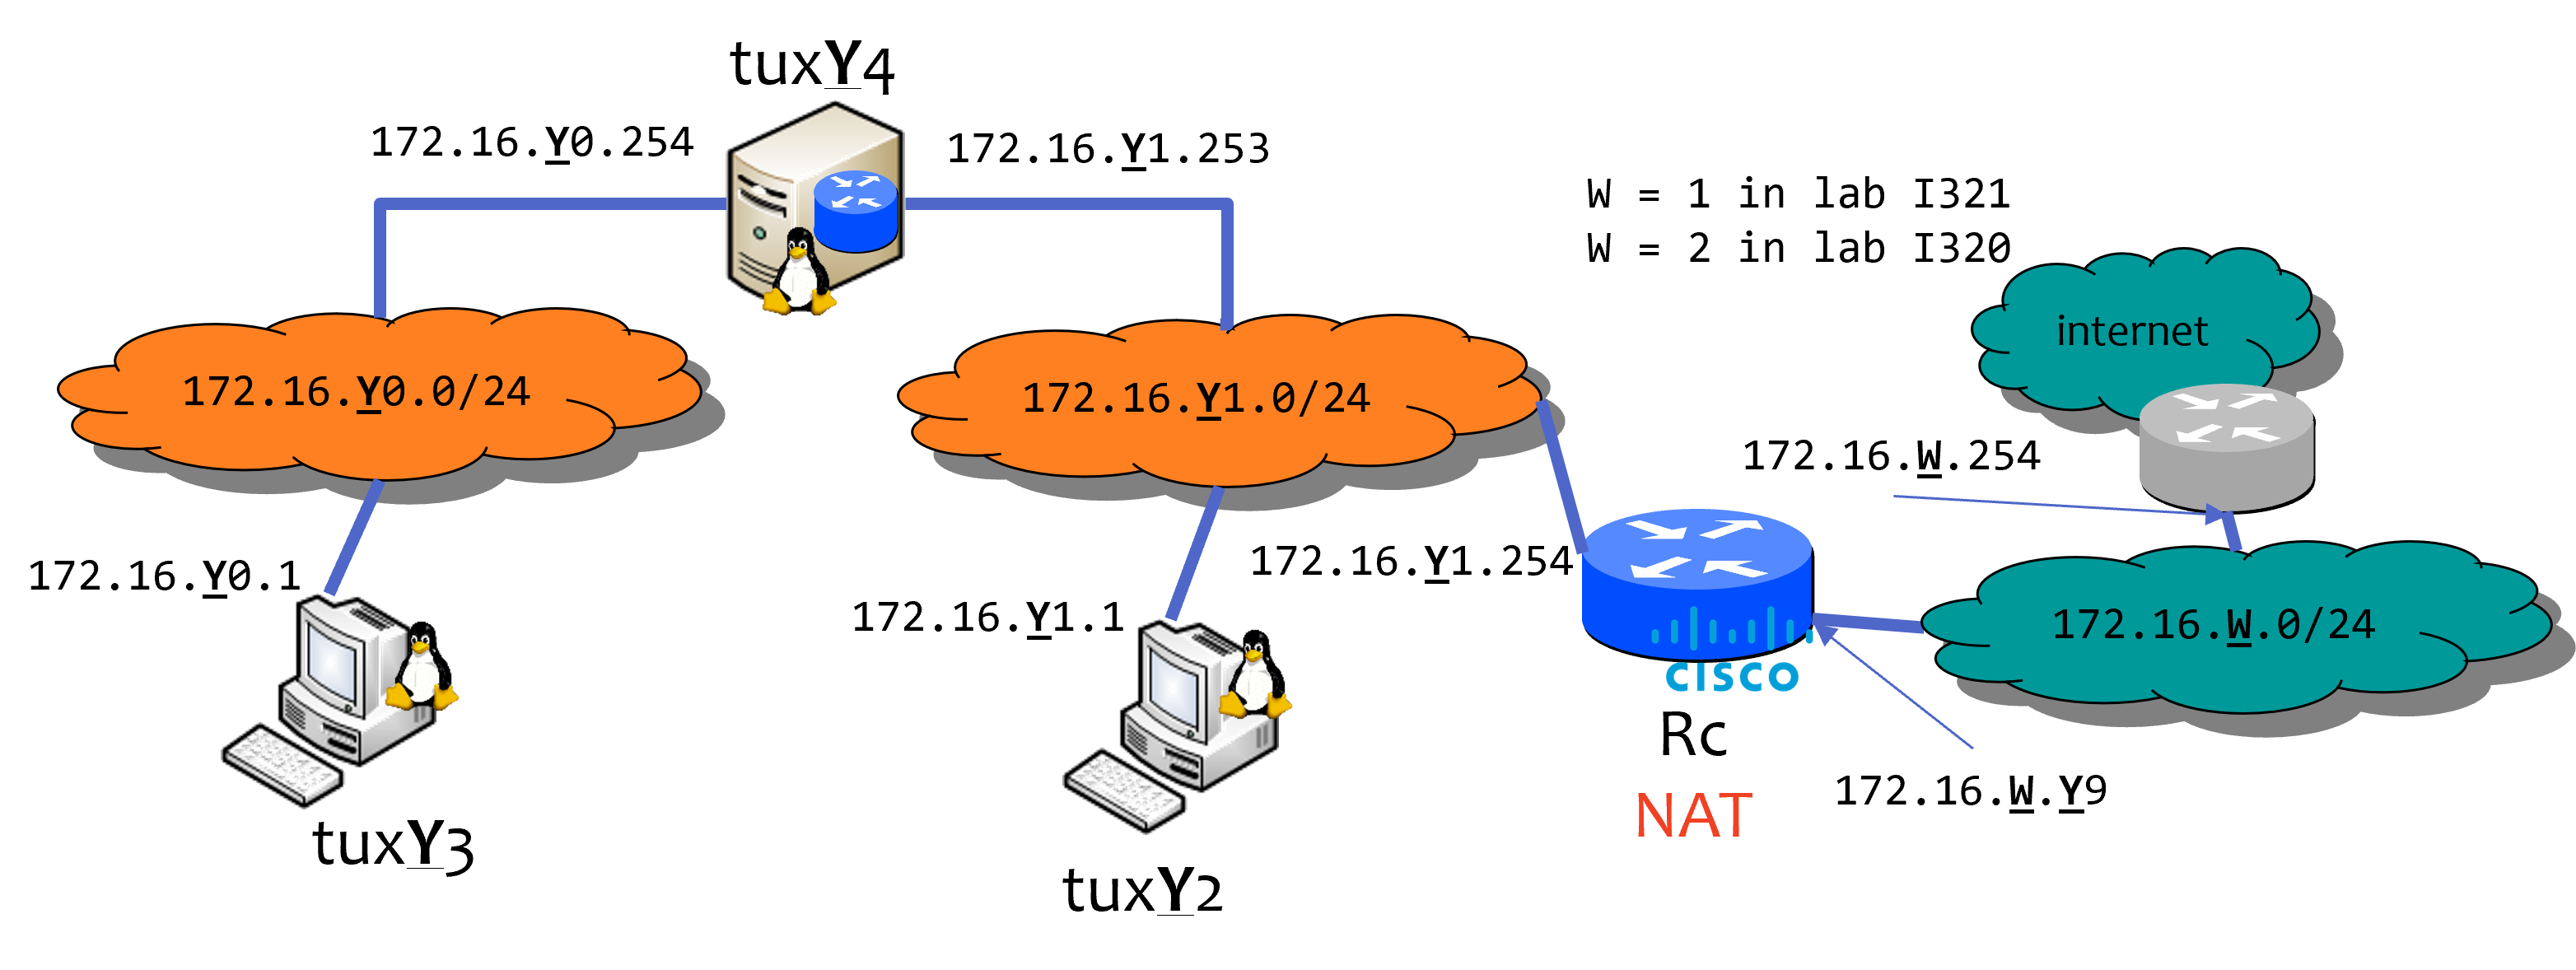
\includegraphics[width=.5\linewidth]{img/net-complete-noFTP.png}
  \caption{Estrutura da rede}
\end{figure}

\subsubsection{Questões}

\paragraph{Que rotas há nos tuxes? Qual é o seu significado?}

\paragraph{Tux52}

\begin{center}
    \begin{tabular}{ c c c }
        \textbf Destino     & \textbf Gateway       & \textbf Máscara de subrede \\ \hline
        0.0.0.0     & 172.16.11.254 & 0.0.0.0            \\
        172.16.11.0 & 0.0.0.0       & 255.255.255.0      \\
        172.16.10.0 & 172.16.11.253 & 255.255.255.0     
    \end{tabular}
\end{center}

\begin{itemize}
    \item Primeira entrada: é o endereço default, indica que todos os pacotes que não tenham match em qualquer outra rota devem ser enviados para o endereço IP 172.16.11.254 neste caso o endereço do router, que encaminhará o pacote para a internet.
    \item Segunda entrada: significa que qualquer pacote que tenha como destino a VLAN11 deve ser tratado localmente (0.0.0.0) uma vez que já atingiu a VLAN correta e não tem de ser encaminhado.
    \item Terceira entrada: significa que qualquer pacote que tenha como destino a VLAN10 deve ser enviado para o endereço 172.16.11.253 o endereço da interface do tux14 na VLAN11, uma vez que este computador é a interface entre as duas VLAN e saberá encaminhar o pacote corretamente.
\end{itemize}

\paragraph{Tux53}

\begin{center}
    \begin{tabular}{ c c c }
    \textbf Destino     & \textbf Gateway       & \textbf Máscara de subrede \\ \hline
    0.0.0.0     & 172.16.10.254 & 0.0.0.0            \\
    172.16.10.0 & 0.0.0.0       & 255.255.255.0      \\
    172.16.11.0 & 172.16.10.254 & 255.255.255.0     
    \end{tabular}
\end{center}

\begin{itemize}
    \item Primeira entrada: é o endereço default, indica que todos os pacotes que não tenham match em qualquer outra rota devem ser enviados para o endereço IP 172.16.10.254 neste caso o endereço do tux14, que encaminhará o pacote para o router.
    \item Segunda entrada: significa que qualquer pacote que tenha como destino a VLAN10 deve ser tratado localmente (0.0.0.0) uma vez que já atingiu a VLAN correta e não tem de ser encaminhado.
    \item Terceira entrada: significa que qualquer pacote que tenha como destino a VLAN11 deve ser enviado para o endereço 172.16.10.254 o endereço da interface do tux14 na VLAN10, uma vez que este computador é a interface entre as duas VLAN e saberá encaminhar o pacote corretamente.
\end{itemize}

\paragraph{Tux54}

\begin{center}
    \begin{tabular}{lll}
    \textbf Destino     & \textbf Gateway       & \textbf Máscara de subrede \\ \hline
    0.0.0.0     & 172.16.11.254 & 0.0.0.0            \\
    172.16.10.0 & 0.0.0.0       & 255.255.255.0      \\
    172.16.11.0 & 0.0.0.0       & 255.255.255.0     
    \end{tabular}
\end{center}

\begin{itemize}
    \item Primeira entrada: é o endereço default, indica que todos os pacotes que não tenham match em qualquer outra rota devem ser enviados para o endereço IP 172.16.11.254 neste caso o endereço do router, que encaminhará o pacote para a internet.
    \item Segunda entrada: significa que qualquer pacote que tenha como destino a VLAN10 deve ser tratado localmente (0.0.0.0) uma vez que já atingiu a VLAN correta e não tem de ser encaminhado.
    \item Terceira entrada: significa que qualquer pacote que tenha como destino a VLAN11 deve ser tratado localmente (0.0.0.0) uma vez que já atingiu a VLAN correta e não tem de ser encaminhado.
\end{itemize}

\paragraph{Que informação contém uma entrada da forwarding table?}

Uma entrada na forwarding table contém os seguintes dados:
\begin{itemize}
    \item Endereço de destino para uma subrede (Destination) 
    \item Máscara de subrede(Genmask)
    \item Endereço do próximo salto (Gateway)
    \item Flags associadas com ACL
    \item Métrica associada à ligação. É escolhida a entrada com a métrica menor
    \item Número de rotas que se referem aquela entrada, este valor não é usado pelo kernel Linux (Ref)
    \item Coluna com número de consultas à rota (Use)
    \item Interface de comunicação (Iface)
\end{itemize}


\paragraph{Que mensagens ARP, e endereços MAC, são observados e porquê?}

Ao fazer ping do tux13 para o tux12 capturando pacotes nas duas interfaces são observados os seguintes pacotes ARP.

Primeiro é observado um pacote que pede que o endereço MAC do IP 172.16.10.254 seja envidado para 172.16.10.1, o endereço MAC observado é 00:21:5a:61:2f:24 (Figure 24).
Isto acontece porque o tux13 está a encontrar a interface do tux14 que encaminhará o pacote enviado pelo ping para o tux12, o endereço MAC de resposta corresponde à interface eth0 de tux14.

Em seguida na mesma interface é observado o pacote ARP que pede que o endereço MAC de 172.16.10.1 seja enviado para 172.16.10.254 (Figure 26).
Isto acontece porque o tux14 necessita do endereço MAC da interface do tux13 para encaminhar a resposta do tux12 ao ping. O endereço MAC observado é 00:21:5a:61:2d:ef o endereço de eth0 do tux13.

Já em eth1 do tux14 acontece algo semelhante, o tux14 pergunta qual o endereço MAC do tux12 (Figure 23) para lhe poder encaminhar o pacote de PING e este responde com 00:21:5a:61:2e:c3, o endereço MAC de eth0 do tux12. Em seguida o tux12 pede o endereço MAC de eth1 de tux14 (Figure 25) para lhe poder enviar a resposta a PING para que esta seja encaminhada a tux13. O tux14 responde com 00:c0:df:04:20:99 o endereço MAC de eth1 do tux14.

\paragraph{Quais são os endereços IP e MAC associados aos pacotes ICMP e porquê?}

Quando o tux13 envia o pacote ICMP para o tux12 o endereço IP de origem é 172.16.10.1 o endereço de tux13 e o de destino 172.16.11.1, o endereço de tux12. O endereço MAC de origem é o endereço 00:21:5a:61:2d:ef o enderço da interface de tux13 e o de destino 00:21:5a:61:2f:24, o endereço MAC de eth0 de tux14. Isto acontece porque o endereço MAC de destino é sempre o endereço da próxima interface e não o endereço MAC correspondente ao destino final. Como os pacotes têm de passar por tux4 este é o endereço MAC de destino. O mesmo acontece com os pacotes de resposta, os endereços IP são os endereços da origem neste caso o tux12 e o de destino é o de tux13. Já o endereço MAC de origem é o endereço de eth0 de tux14 e o de destino eth0 de tux13.

Na interface eth1 de tux4 acontece algo semelhante. Os pacotes enviados por tux13 têm o seu endereço IP como endereço IP de origem e o endereço IP de tux12 como destino. Já o endereço MAC de origem é o de eth1 de tux14 e o de destino o de eth0 de tux12. O contrário acontece com os pacotes de resposta, estes possuem como endereço de IP de origem o endereço de tux12 e o de destino o de tux13. Mas o endereço MAC de origem é eth0 de tux12 e o de destino eth1 de tux14.

\paragraph{Quais são os caminhos seguidos pelos pacotes nas experiências realizadas e porquê?}

\begin{itemize}
    \item \textbf{Router CISCO para tux12 - } O caminho seguido é router $\rightarrow$ tux12 pois estes encontram-se na mesma VLAN e podem comunicar diretamente
    \item \textbf{Router CISCO para tux13 - } O caminho seguido é router $\rightarrow$ tux14 $\rightarrow$ tux13 pois o router encontra-se na VLAN11 e o tux13 na VLAN10 por isso os pacotes enviados têm de ser enviados primeiro para tux14 
    \item \textbf{Router CISCO para tux14 - } A comunicação é direta uma vez que ambos têm interfaces conectadas à mesma VLAN
    \item \textbf{Router CISCO para a 172.16.1.254 - } A comunicação pode ser feita diretamente pois o router têm uma interface ligada à VLAN onde está a máquina de endereço 172.16.1.254.
    \item \textbf{Tux13 para 172.16.1.254 - } O caminho seguido é tux13 $\rightarrow$ tux14 $\rightarrow$ router $\rightarrow$ 172.16.1.254, isto acontece porque o tux13 não tem ligação direta a 172.16.1.254 nem ao router por isso o pacote tem de ser enviado ao tux14 que o encaminhará para o router. O router por sua vez encaminha o pacote para 172.16.1.254.
    \item \textbf{Tux13 para 104.17.113.188 - } O caminho seguido é  tux13 $\rightarrow$ tux14 $\rightarrow$ router $\rightarrow$ 172.16.1.254 $\rightarrow$ ... $\rightarrow$ 104.17.113.188, a justificação para o encaminhamento até 172.16.1.254 é a mesma que na comunicação anterior, no entanto após atingir 172.16.1.254 o pacote será encaminhado para a Internet, aí fará um caminho que desconhecemos até atingir 104.17.113.188. 
\end{itemize}

 

\input{Conclusões}
\section{Bibliografia}

\href{https://man7.org/linux/man-pages/man8/route.8.html}{route command Man Pages}

\href{https://man7.org/linux/man-pages/man8/ifconfig.8.html}{ifconfig command Man Pages}

\href{https://linux.die.net/man/8/ip}{ip command Man Pages}

\href{https://www.cisco.com/c/en/us/td/docs/routers/access/1900/software/configuration/guide/Software_Configuration/routconf.html}{Cisco Basic Router Configuration}

\newpage
\section{Anexo 1}

\paragraph{Modules}

\begin{itemize}
    \item \textbf{application} - camada de aplicação
    \item \textbf{main} - interpretação dos argumentos de chamada
    \item \textbf{file} - interpretação e validação do nome de ficheiro dado
    \item \textbf{error} - simulação de erros e do tempo de propagação
    \item \textbf{state} machine - máquina de estados
    \item \textbf{data} link - protocolo de ligação de dados
    \item \textbf{macros} - constantes
\end{itemize}

\subsection{application.c}

\begin{lstlisting}[language=C, caption=application.c]
#include <stdio.h>
#include <unistd.h>
#include <fcntl.h>
#include <sys/stat.h>
#include <string.h>
#include <stdlib.h>
#include <stdint.h>
#include "file.h"
#include "data_link.h"
#include "application.h"

typedef struct {
    int file_descriptor;
    size_t transfer_file_size;
    ConnectionType status;
    char* transfer_file_name;
    char* transfer_file_dir;
    char* transfer_file_path;
} ApplicationLayer;

ApplicationLayer app_data;

int receiver(char* port_path);
int transmitter(char* port_path);

// RECEIVER AUX
size_t write_data_packet(uint8_t* data_packet, int fd, int* packet_no);
void parse_control_packet(uint8_t* packet);
int open_transfer_file();

// TRANSMITTER AUX
uint8_t* build_control_packet(size_t* control_packet_size, char* file_name);
size_t read_data_packet(int packetNo, uint8_t* data_packet, int fd, int bytes_read);
int read_file(char* file_path, uint8_t* buffer, size_t size);


void init_app(ConnectionType connection_type, char* file_path, char* serial_path) {
    app_data.transfer_file_name = calloc(FILE_NAME_SIZE, sizeof(char));
    app_data.transfer_file_dir = calloc(DIR_PATH_SIZE, sizeof(char));
    app_data.status = connection_type;
    
    path_parser(file_path, app_data.transfer_file_dir, app_data.transfer_file_name);

    if (connection_type == TRANSMITTER) {
        app_data.transfer_file_path = file_path;
        transmitter(serial_path);
    }
    if (connection_type == RECEIVER) {
        app_data.transfer_file_path = calloc(DIR_PATH_SIZE + FILE_NAME_SIZE, sizeof(char));
        receiver(serial_path);
        free(app_data.transfer_file_path);
    }

    free(app_data.transfer_file_dir);
    free(app_data.transfer_file_name);
}

void parse_control_packet(uint8_t* packet) {
    int i = 1;
    if (packet[i++] == 0x00) { // Filesize
        size_t file_size = 0;
        int n_bytes = (int) packet[i++];
        n_bytes--;
        while(n_bytes >= 0) {
            file_size += (size_t) packet[i++] << (n_bytes * 8);
            n_bytes--;
        }
        app_data.transfer_file_size = file_size;
    } else {
        fprintf(stderr, "Error in application - parse_control_packet: unexpected structure of the control_packet\n");
        exit(1);
    }
    if (packet[i++] == 0x01) { // Filename
        int n_bytes = (int) packet[i++];
        if (strlen(app_data.transfer_file_name) == 0) {
            strncpy(app_data.transfer_file_name, (char*) packet + i, n_bytes);
        }
        strncpy(app_data.transfer_file_path, app_data.transfer_file_dir, DIR_PATH_SIZE);
        strcat(app_data.transfer_file_path, app_data.transfer_file_name);
    } else {
        fprintf(stderr, "Error in application - parse_control_packet: unexpected structure of the control_packet\n");
        exit(1);
    }
}

size_t write_data_packet(uint8_t* data_packet, int fd, int* packet_no) {

    size_t packet_size = (size_t) (data_packet[2] << 8) + data_packet[3];
    if (*packet_no == (int) data_packet[1]) {
        (*packet_no)++;
    } else {
        fprintf(stderr, "Packet sequence number incorrect! Missed a packet\n");
        (*packet_no) = (int) data_packet[1] + 1;
    }

    if ((write(fd, data_packet + 4, packet_size * sizeof(uint8_t))) != packet_size) {
        perror("Error in application - write_data_packet");
        exit(1);
    }
    return packet_size;
}

int receiver(char* port_path) {

    int newFileDescriptor, packet_no = 0;
    size_t bytes_received = 0;
    bool fileOpen = false;
    uint8_t *data_packet;
    data_packet = calloc(MAX_PACKET_SIZE, sizeof(uint8_t));

    // OPEN
    if((app_data.file_descriptor = llopen(port_path, RECEIVER)) == -1) exit(1);

    printf("Receiver - connection established\n");
    
    while (true) {
        // READ
        if (llread(app_data.file_descriptor, data_packet, MAX_PACKET_SIZE) == -1) exit(1);
        if (data_packet[0] == 0x01) {
            bytes_received += write_data_packet(data_packet, newFileDescriptor, &packet_no);
            printf("Receiver - packet %d received\n", (int) data_packet[1]);
        } else if (data_packet[0] == 0x02) {
            parse_control_packet(data_packet);
            if (file_exists(app_data.transfer_file_dir, app_data.transfer_file_name)) {
                fprintf(stderr, "Error in application - receiver: file already exists\n");
                exit(1);
            }
            newFileDescriptor = open_transfer_file();
            fileOpen = true;

        } else if (data_packet[0] == 0x03) {
            // CLOSE
            if ((llclose(app_data.file_descriptor)) != 0) exit(1);
            printf("Receiver - connection cut\n");
            break;
        } else {
            fprintf(stderr, "Error in application - receiver: C byte value invalid\n");
            exit(1);
        }
    }

    if (bytes_received != app_data.transfer_file_size) {
        fprintf(stderr, "File size does not correspond to the expected\n");
    }

    if (fileOpen) {
        if ((close(newFileDescriptor) == -1)) {
            perror("Error in application - receiver");
            exit(1);
        }
    }
    free(data_packet);
    
    return 0;
}

size_t read_data_packet(int packetNo, uint8_t* data_packet, int fd, int bytes_read) {
    size_t bytes_to_write = (MAX_PACKET_SIZE > (app_data.transfer_file_size - bytes_read + 4)) ? (app_data.transfer_file_size - bytes_read) : MAX_PACKET_SIZE - 4; // In case of the file being in its end
    data_packet[0] = 0x01;
    data_packet[1] = (uint8_t) packetNo;
    data_packet[2] = (uint8_t) (bytes_to_write & 0xFF00) >> 8; // Amount of data
    data_packet[3] = (uint8_t) bytes_to_write & 0x00FF;
    if ((read(fd, data_packet + 4, bytes_to_write * sizeof(uint8_t))) != bytes_to_write) {
        perror("Error in application - read_data_packet");
        exit(1);
    }
    return bytes_to_write + 4;
}

uint8_t* build_control_packet(size_t* control_packet_size, char* file_name) {
    size_t file_name_size = strlen(file_name) + 1; //To actually copy \0

    if (file_name_size > MAX_PACKET_SIZE - 13) {
        fprintf(stderr, "Error in application - build_control_packet: filename too big\n");
        exit(1);
    }

    *control_packet_size = file_name_size + 13;
    uint8_t* buffer = calloc((*control_packet_size), sizeof(uint8_t));

    buffer[0] = 0x02; // C
    buffer[1] = 0; // T
    buffer[2] = (uint8_t) sizeof(app_data.transfer_file_size); // L
    buffer[3] = (app_data.transfer_file_size & 0xFF00000000000000) >> 56; // filesize
    buffer[4] = (app_data.transfer_file_size & 0x00FF000000000000) >> 48;
    buffer[5] = (app_data.transfer_file_size & 0x0000FF0000000000) >> 40;
    buffer[6] = (app_data.transfer_file_size & 0x000000FF00000000) >> 32;
    buffer[7] = (app_data.transfer_file_size & 0x00000000FF000000) >> 24;
    buffer[8] = (app_data.transfer_file_size & 0x0000000000FF0000) >> 16;
    buffer[9] = (app_data.transfer_file_size & 0x000000000000FF00) >> 8;
    buffer[10] = app_data.transfer_file_size & 0x00000000000000FF;
    buffer[11] = 1; // T
    buffer[12] = (uint8_t) (sizeof(char) * file_name_size); // L
    memcpy((char*) buffer + 13, file_name, file_name_size); // filename
    return buffer;
}

int transmitter(char* port_path) {
    uint8_t *control_packet, *data_packet;
    struct stat s;
    size_t control_packet_size, bytes_read = 0, bytes_written;
    int packet_no = 0, oldFileDescriptor;

    if (stat(app_data.transfer_file_path, &s) == -1) {
        perror("Error in application - transmitter - stat");
        exit(1);
    }
    app_data.transfer_file_size = s.st_size;
    data_packet = calloc(MAX_PACKET_SIZE, sizeof(uint8_t));

    oldFileDescriptor = open_transfer_file();

    // OPEN
    if( (app_data.file_descriptor = llopen(port_path, TRANSMITTER)) == -1) exit(1);
    control_packet = build_control_packet(&control_packet_size, app_data.transfer_file_name);

    printf("Transmitter - connection established\n");

    // START
    if ((llwrite(app_data.file_descriptor, control_packet, control_packet_size)) == -1) exit(1); 

    printf("Transmitter - transmition begun\n");

    // WRITING
    while (bytes_read < app_data.transfer_file_size) {
        packet_no++;
        bytes_written = read_data_packet(packet_no, data_packet, oldFileDescriptor, bytes_read);
        bytes_read += bytes_written - 4;
        if ((llwrite(app_data.file_descriptor, data_packet, bytes_written)) == -1) exit(1);
        printf("Transmitter - packet %d sent\n", packet_no);
    }

    // FINISH
    control_packet[0] = 0x03;
    if ((llwrite(app_data.file_descriptor, control_packet, control_packet_size)) == -1) {
        fprintf(stderr, "Error in application - transmitter - fatal error when writting control packet\n");
        exit(1);
    } 

    printf("Transmitter - transmition ended\n");

    // CLOSE
    if ((llclose(app_data.file_descriptor)) != 0) exit(1);

    printf("Transmitter - connection cut\n");

    if ((close(oldFileDescriptor) == -1)) {
        perror("Error in application - transmitter");
        exit(1);
    }

    free(data_packet);
    free(control_packet);  

    return 0;
}

int open_transfer_file() {
    int fd;

    switch (app_data.status) {
        case TRANSMITTER: {
            if ((fd = open(app_data.transfer_file_path, O_RDONLY)) == -1) {
                perror("Error in application - transmitter - open_transfer_file");
                exit(1);
            }
            break;
        }
        case RECEIVER: {
            if ((fd = creat(app_data.transfer_file_path, S_IRUSR | S_IWUSR | S_IRGRP | S_IROTH)) == -1) {
                perror("Error in application - receiver - open_transfer_file");
                exit(1);
            }
            break;
        }

        default: {
            fprintf(stderr, "Error in application - open_transfer_file: wrong type of connection\n");
            exit(1);
        }
    }
    return fd;
}
\end{lstlisting}

\subsection{application.h}

\begin{lstlisting}[language=C, caption=application.h]
#pragma once

#include "macros.h"

void init_app(ConnectionType connection_type, char* file_path, char* serial_path);

\end{lstlisting}

\subsection{main.c}

\begin{lstlisting}[language=C, caption=main.c]
#include <stdio.h>
#include <stdlib.h>
#include <stdbool.h>
#include <getopt.h>
#include <time.h>
#include "error.h"
#include "state_machine.h"
#include "application.h"

void print_cmd_args() {
    printf("Usage: \n");
    printf("    rcompy -r/-t --file <argument> --serial_port <argument> [--fer <argument> --t_prop <argument> --help]\n");
    printf("Options: \n");
    printf("    -r               Receiver mode\n");
    printf("    -t               Transmitter mode\n");
    printf("    -f --file        Choose destination if receiver or source if transmitter\n");
    printf("    -s --serial_port Choose serial port path\n");
    printf("    -z --header_error_ratio        Choose error generation probability in information packets\n");
    printf("    -x --data_error_ratio         Choose error generation probability in information packets\n");
    printf("    -p --t_prop      Choose propagation delay in milliseconds\n");
    printf("    -h --help        Show this help message\n");
}

// Just parsing
int main(int argc, char** argv) {
    
    srandom(time(NULL));
    struct option options[] = {
        {"file", required_argument, 0, 'f'},
        {"serial_port", required_argument, 0, 's'},
        {"header_error_ratio", required_argument, 0, 'z'},
        {"data_error_ratio", required_argument, 0, 'x'},
        {"t_prop", required_argument, 0, 'p'},
        {"help", required_argument, 0, 'h'},
        {0, 0, 0, 0}
    };

    bool is_trans, is_rec, had_file_path, had_serial_path, had_header_error, had_data_error, had_tprop;
    is_trans = is_rec = had_file_path = had_serial_path = had_header_error = had_data_error = had_tprop = false;

    char* file_path;
    char* serial_port_path;
    int t_prop = 0;
    double header_error = 0;
    double data_error = 0;

    int c = 0;
    int opt_index = 0;
    while((c = getopt_long(argc, argv, "htrf:p:x:z:s:", options, &opt_index)) != -1) {
        switch (c) {
            case 't': {
                is_trans = true;
                if (is_rec) {
                    print_cmd_args();
                    return 1;
                }
                break;
            }
            case 'r': {
                is_rec = true;
                if (is_trans) {
                    print_cmd_args();
                    return 1;
                }
                break;
            }
            case 'f': {
                if (had_file_path) {
                    print_cmd_args();
                    return 1;
                }
                had_file_path = true;
                file_path = optarg;
                break;
            }
            case 's': {
                if (had_serial_path) {
                    print_cmd_args();
                    return 1;
                }
                had_serial_path = true;
                serial_port_path = optarg;
                break;
            }
            case 'p': {
                if (had_tprop) {
                    print_cmd_args();
                    return 1;
                }
                had_tprop = true;
                t_prop = atoi(optarg);
                break;
            }
            case 'z': {
                if (had_header_error) {
                    print_cmd_args();
                    return 1;
                }
                had_header_error = true;
                header_error = strtod(optarg, NULL);
                break;
            }
            case 'x': {
                if (had_data_error) {
                    print_cmd_args();
                    return 1;
                }
                had_data_error = true;
                data_error = strtod(optarg, NULL);
                break;
            }
            case 'h': {
                print_cmd_args();
                return 1;
            }
            default: {
                print_cmd_args();
                return 1;
            }
        }
    }
    if (!had_file_path || !had_serial_path || (!is_rec && !is_trans)) {
        print_cmd_args();
        return 1;
    }

    set_error_rates(header_error, data_error);
    set_prop_time(t_prop);
    init_app(is_rec ? RECEIVER : TRANSMITTER, file_path, serial_port_path);

    return 0;
}
\end{lstlisting}

\subsection{data \textunderscore link.c}

\begin{lstlisting}[language=C, caption=data_link.c]
#include <unistd.h>
#include <stdio.h>
#include <string.h>
#include <fcntl.h>
#include <strings.h>
#include <termios.h>
#include <stdbool.h>
#include "data_link.h"
#include "alarm.h"
#include "state_machine.h"
#include "macros.h"


static struct termios old_terminal;
static struct LinkLayerData link_layer_data;
static uint8_t* aux_buffer;
static bool alarm_called = false;

int setup_terminal(int fd);
int restore_terminal(int fd);

int assemble_supervision_frame(FrameType frame_type, ConnectionType connection_type, uint8_t* frame_buffer);
uint32_t assemble_information_frame(uint8_t* packet_data, size_t packet_size, uint8_t* frame, uint8_t frame_number);
int write_buffer(int fd, uint8_t* buffer, size_t length, FrameType expected_response);
bool validBCC2(uint8_t bcc2, uint8_t* buffer, size_t buffer_size);
uint8_t compute_bcc2(uint8_t* buffer, size_t buffer_size);

int establish_transmitter_connection(int fd);
int wait_transmitter_connection(int fd);
int disconnect_transmitter(int fd);
int disconnect_receiver(int fd);

void dl_alarm_callback() {
    alarm_called = true;
}

int llopen(char* port, ConnectionType role) {

    int fd = 0;
    alarm_called = false;

    // Configure port
    snprintf(link_layer_data.port, sizeof(char)*MAX_PORT_SIZE, "%s", port);
    link_layer_data.role = role;
    link_layer_data.baud_rate = BAUDRATE;
    link_layer_data.num_transmissions = NUM_TX;
    link_layer_data.timeout = TIMEOUT;

    if ((link_layer_data.frame = calloc(MAX_FRAME_SIZE, sizeof(uint8_t))) == NULL) {
        return -1;
    }
    if ((aux_buffer = calloc(MAX_FRAME_SIZE + 1, sizeof(uint8_t))) == NULL) {
        return -1;
    }

    fd = open(link_layer_data.port, O_RDWR | O_NOCTTY );
    if (fd < 0) {
        perror("Error in data_link - llopen - opening port");
        return -1;
    } 

    if (setup_terminal(fd) == -1) {
        perror("Error in data_link - llopen");
        return -1;
    }

    if (setup_alarm_handler() == -1) {
        fprintf(stderr, "Error in data_link - llopen: setting up alarm handler\n");
        return -1;
    }

    if (subscribe_alarm(dl_alarm_callback) == -1) { // Subscribing a specific function to be called in alarm
        fprintf(stderr, "Error in data_link - llopen: subscribing alarm event\n");
        return -1;
    }

    switch(role) {
        case TRANSMITTER: {
            if ((establish_transmitter_connection(fd)) == -1) return -1;
            break;
        }
        case RECEIVER: {
            if ((wait_transmitter_connection(fd)) == -1) return -1;
            break;
        }
        default: {
            fprintf(stderr, "Error in data_link - llopen: tried to open a connection with invalid role\n");
            return -1;
        }
    }

    return fd;   
}

int llclose(int fd) {
    if (link_layer_data.role == TRANSMITTER) {
        disconnect_transmitter(fd);
    } else if (link_layer_data.role == RECEIVER) {
        disconnect_receiver(fd);
    }
    if (restore_terminal(fd) == -1) {
        perror("Error in data_link - llclose");
        return -1;
    }
    if (restore_alarm_handler() == -1) {
        fprintf(stderr, "Error in data_link - llclose: restoring alarm handlers\n");
        return -1;
    }
    free(aux_buffer);
    free(link_layer_data.frame);
    return close(fd);
}

int llwrite(int fd, uint8_t* packet, size_t packet_length) {
    static uint8_t package_to_send = 0;
    uint8_t frame_length;
    FrameType expected_response;

    // Numero de sequência
    if (package_to_send == 0) {
        expected_response = RR_1;
        frame_length = assemble_information_frame(packet, packet_length, link_layer_data.frame, 0);
    } else {
        expected_response = RR_0;
        frame_length = assemble_information_frame(packet, packet_length, link_layer_data.frame, 1);
    }

    // Writing
    int res = write_buffer(fd, link_layer_data.frame, frame_length, expected_response);
    if ( res == -2) {
        fprintf(stderr, "Error in data_link - llwrite: no. tries exceeded\n");
        return -1;
    } else if ( res == -1) {
        perror("Error in data_link - llwrite");
        return -1;
    } else if ( res != frame_length) {
        fprintf(stderr, "Error in data_link - llwrite: no. bytes written not matching expected\n");
        return -1;
    }
    package_to_send = package_to_send ? 0 : 1;
    return res;
}

/*
    This function reads into a buffer a packet that was read from the serial port
    fd -> Serial port file descriptor
    buffer -> Buffer that will receive the packet
    max_buffer_size -> Max size of buffer variable, used to check if a packet can fit into the provided buffer
*/
int llread(int fd, uint8_t* buffer, size_t max_buffer_size) {
    if (max_buffer_size < MAX_PACKET_SIZE) {

        fprintf(stderr, "Error in data_link - llread: provided buffer does not meet size requirements\n");
        return -1;
    }

    size_t frame_size;
    static uint8_t expected_package;
    uint8_t response_frame[SUPV_FRAME_SIZE];
    StateMachineResult new_frame;
    bool valid_frame = false;

    while(!valid_frame) {

        new_frame = read_frame(fd, link_layer_data.frame, MAX_FRAME_SIZE);
        frame_size = destuff(link_layer_data.frame, new_frame.packet_size, aux_buffer, MAX_PACKET_SIZE + 1);

        if (frame_size == 0) {
            fprintf(stderr, "Error in data_link - llread: destuffing packet unsuccessfull\n");
            return -1;
        }
        uint8_t bcc2 = aux_buffer[--frame_size];

        // Error
        if (new_frame.frame_type != expected_package || !validBCC2(bcc2, aux_buffer, frame_size)) {
            if (assemble_supervision_frame(expected_package ? REJ_1 : REJ_0, RECEIVER, response_frame) == -1) return -1;
        } else {
            memcpy(buffer, aux_buffer, frame_size);
            if (assemble_supervision_frame(expected_package ? RR_0 : RR_1, RECEIVER, response_frame) == -1) return -1;
            valid_frame = true;
        }
        if (write(fd, response_frame, SUPV_FRAME_SIZE) != 5) {
            fprintf(stderr, "Error in data_link - llread: did not write response frame correctly");
            return -1;
        }
    }

    expected_package = expected_package ? 0 : 1;
    return frame_size;
}

int setup_terminal(int fd) {
    struct termios new_terminal;

    if ( tcgetattr(fd, &old_terminal) == -1) {
      return -1;
    }

    bzero(&new_terminal, sizeof(new_terminal));
    new_terminal.c_cflag = link_layer_data.baud_rate | CS8 | CLOCAL | CREAD;
    new_terminal.c_iflag = IGNPAR;
    new_terminal.c_oflag = 0;
    new_terminal.c_lflag = 0;

    new_terminal.c_cc[VTIME] = VTIME_VALUE;
    new_terminal.c_cc[VMIN] = VMIN_VALUE;

    tcflush(fd, TCIOFLUSH);

    if ( tcsetattr(fd,TCSANOW,&new_terminal) == -1) {
      return -1;
    }
     
    return 0;
}

int restore_terminal(int fd) {
    if (tcsetattr(fd,TCSANOW,&old_terminal) == -1) {
      return -1;
    }
    return 0;
}

int assemble_supervision_frame(FrameType frame_type, ConnectionType connection_type, uint8_t* frame_buffer) {
    frame_buffer[0] = FLAG;
    switch (connection_type) {
        case TRANSMITTER: {
            frame_buffer[1] = 0x03;
            if (frame_type == UA) {
                frame_buffer[1] = 0x01;
            } 
            if (frame_type == SET || frame_type == DISC || frame_type == UA) {
                frame_buffer[2] = frame_type;
            } else {
                fprintf(stderr, "Error: Data_link - assemble_supervision_frame - invalyd frame_type: %x\n", frame_type);
                return -1; //Invalid frame_type for this function
            }
            break;
        }
        case RECEIVER: {
            frame_buffer[1] = 0x03;
            if (frame_type == DISC) {
                frame_buffer[1] = 0x01;
            } 
            if (frame_type == UA || frame_type == DISC || frame_type == RR_0 || frame_type == RR_1 || frame_type == REJ_0 || frame_type == REJ_1) {
                frame_buffer[2] = frame_type;
            } else {
                fprintf(stderr, "Error: Data_link - assemble_frame - invalyd frame_type\n");
                return -1; //Invalid frame_type for this function
            }
            break;
        }
    }
    frame_buffer[3] = frame_buffer[1] ^ frame_buffer[2];
    frame_buffer[4] = FLAG;
    return 0;
}

uint32_t assemble_information_frame(uint8_t* packet_data, size_t packet_size, uint8_t* frame, uint8_t frame_number) {
    size_t frame_size = 4;
    frame[0] = FLAG;
    frame[1] = 0x03;
    frame[2] = frame_number;
    frame[3] = frame[1] ^ frame[2];
    frame_size = stuff(packet_data, packet_size, frame, frame_size);
    uint8_t bcc2[2];
    bcc2[0] = compute_bcc2(packet_data, packet_size);
    frame_size = stuff(bcc2, 1, frame, frame_size);
    frame[frame_size++] = FLAG;
    return frame_size;
}

uint32_t stuff(uint8_t* packet, size_t length, uint8_t* frame, size_t occupied_bytes) {
    size_t stuffed_length = occupied_bytes;

    int new_buffer_i = occupied_bytes;

    for (int i = 0; i < length; i++) {
        uint8_t byte = packet[i];
        if (byte == FLAG || byte == ESC_HEX) {
            frame[new_buffer_i++] = ESC_HEX;
            frame[new_buffer_i++] =  byte ^ STUFF_XOR_HEX;
            stuffed_length++;
        } else {
            frame[new_buffer_i++] = byte;
        }
        stuffed_length++;
    }
    return stuffed_length;
}

uint32_t destuff(uint8_t* stuffed_packet, size_t stuffed_length, uint8_t* unstuffed_packet, size_t max_unstuffed_packet_size) {
    size_t unstuffed_length = stuffed_length;

    int64_t new_buffer_i = 0;

    for (int i = 0; i < stuffed_length; i++) {
        uint8_t byte = stuffed_packet[i];
        if (new_buffer_i >= max_unstuffed_packet_size) {
            fprintf(stderr, "Error in data_link - destuffing: unstuffed packet is bigger than the destiny buffer! Tried to access %ld on a %ld bytes buffer\n", new_buffer_i, max_unstuffed_packet_size);
            return 0;
        }
        if (byte == ESC_HEX && i < stuffed_length - 1) {
            if (stuffed_packet[i + 1] == (FLAG ^ STUFF_XOR_HEX)) {
                unstuffed_packet[new_buffer_i++] = FLAG;
            } else if (stuffed_packet[i + 1] == (ESC_HEX ^ STUFF_XOR_HEX)) {
                unstuffed_packet[new_buffer_i++] = ESC_HEX;
            }
            unstuffed_length--;
            i++;
        } else {
            unstuffed_packet[new_buffer_i++] = byte;
        }
    }
    return unstuffed_length;
}

int establish_transmitter_connection(int fd) {
    uint8_t supervision_buffer[SUPV_FRAME_SIZE];
    
    if ((assemble_supervision_frame(SET, TRANSMITTER, supervision_buffer)) != 0) {
        return -1;
    }
    int res = write_buffer(fd, supervision_buffer, SUPV_FRAME_SIZE, UA);
    if (res == -2) {
        fprintf(stderr, "Error in data_link - establish_transmitter_connection: no. tries exceeded\n");
        return -1;
    } else if ( res == -1) {
        perror("Error in data_link - disconnect_receiver");
        return -1;
    } else if (res != 5) {
        fprintf(stderr, "Error in data_link - establish_transmitter_connection: no. bytes written not matching expected\n");
        return -1;
    }
    return 0;
}

int wait_transmitter_connection(int fd) {
    StateMachineResult res = read_frame(fd, link_layer_data.frame, MAX_FRAME_SIZE);
    if (res.frame_type == SET) {
        uint8_t supervision_buffer[SUPV_FRAME_SIZE];
        assemble_supervision_frame(UA, RECEIVER, supervision_buffer);
        if (write(fd, supervision_buffer, SUPV_FRAME_SIZE) != 5) {
            fprintf(stderr, "Error in data_link - wait_transmiiter_connection: could no write ACK to transmitter\n");
            return -1;
        }
        return 0;
    } else {
        fprintf(stderr, "Error in data_link - wait_transmiiter_connection: received wrong type of frame\n");
        return -1;
    }
}

int disconnect_transmitter(int fd) {
    uint8_t supervision_buffer[SUPV_FRAME_SIZE];
    assemble_supervision_frame(DISC, TRANSMITTER, supervision_buffer);
    int res = write_buffer(fd, supervision_buffer, SUPV_FRAME_SIZE, DISC); 
    if ( res == -2) {
        fprintf(stderr, "Error in data_link - disconnect_transmitter: no. tries exceeded\n");
        return -1;
    } else if ( res == -1) {
        perror("Error in data_link - disconnect_receiver");
        return -1;
    } else if ( res != 5) {
        fprintf(stderr, "Error in data_link - disconnect_transmitter: no. bytes written not matching expected\n");
        return -1;
    }
    assemble_supervision_frame(UA, TRANSMITTER, supervision_buffer);
    if (write(fd, supervision_buffer, SUPV_FRAME_SIZE) != 5) {
        return -1;
    }
    return 0;
}

int disconnect_receiver(int fd) {

    StateMachineResult res = read_frame(fd, link_layer_data.frame, MAX_FRAME_SIZE);
    if (res.frame_type == DISC) {
        uint8_t supervision_buffer[SUPV_FRAME_SIZE];
        assemble_supervision_frame(DISC, TRANSMITTER, supervision_buffer);
        int res = write_buffer(fd, supervision_buffer, SUPV_FRAME_SIZE, UA); 
        if ( res == -2) {
            fprintf(stderr, "Error in data_link - disconnect_receiver: no. tries exceeded\n");
            return -1;
        } else if ( res == -1) {
            perror("Error in data_link - disconnect_receiver");
            return -1;
        } else if ( res != 5) {
            fprintf(stderr, "Error in data_link - disconnect_receiver: no. bytes written not matching expected\n");
            return -1;
        }
        return 0;
    } else {
        fprintf(stderr, "Error in data_link - disconnect_receiver: unexpected frame type\n");
        return -1;
    }
}

/* Writes a buffer to the serial port and awaits a certain response
    fd -> Serial port file desciptor
    buffer -> buffer to write
    length -> length of the buffer to be written
    expected_response -> expected response sent by the other end of the serial port
*/
int write_buffer(int fd, uint8_t* buffer, size_t length, FrameType expected_response) {
    StateMachineResult res_frame = {};
    int tries = NUM_TX;
    int res = 0;
    while (tries > 0) {
        if((res = write(fd, buffer, length * sizeof(uint8_t))) == -1) return -1; // Writes buffer to serial port
        alarm(3);
        res_frame = read_frame(fd, link_layer_data.frame, MAX_FRAME_SIZE); // Reads response
        if (alarm_called) { // Timeout
            tries--;
            alarm_called = !alarm_called;
            fprintf(stderr, "Alarm called, response timed out, %d tries left\n", tries);
        } else {
            alarm(0);
            if (res_frame.frame_type == expected_response) {
                //Only break if frame received and data was correct
                break;
            }
        }
    }
    if (tries <= 0) { // Timeout limit 
        return -2;
    } else {
        return res;
    }
}

bool validBCC2(uint8_t bcc2, uint8_t* buffer, size_t buffer_size) {
    uint8_t side_bcc2 = compute_bcc2(buffer, buffer_size);
    return ((side_bcc2 ^ bcc2) == 0);
}

uint8_t compute_bcc2(uint8_t* buffer, size_t buffer_size) {
    uint8_t bcc2 = buffer[0];
    for (int i = 1; i < buffer_size; i++) {
        bcc2 ^= buffer[i];
    }
    return bcc2;
}

\end{lstlisting}

\subsection{data \textunderscore link.h}

\begin{lstlisting}[language=C, caption=data_link.h]
#pragma once

#include <stdlib.h>
#include <stdint.h>
#include <stdbool.h>
#include "macros.h"
#include "state_machine.h"

#define MAX_FRAME_SIZE ((MAX_PACKET_SIZE * 2) + 7)

struct LinkLayerData {
    ConnectionType role;
    char port[MAX_PORT_SIZE];
    unsigned int baud_rate;
    unsigned int sequence_number;
    unsigned int timeout;
    unsigned int num_transmissions;
    uint8_t* frame;
} LinkLayerData;

uint32_t stuff(uint8_t* packet, size_t length, uint8_t* frame, size_t occupied_bytes);
uint32_t destuff(uint8_t* stuffed_packet, size_t stuffed_length, uint8_t* unstuffed_packet, size_t max_unstuffed_packet_size);

int llopen(char* port, ConnectionType role);
int llwrite(int fd, uint8_t* buffer, size_t length);
int llread(int fd, uint8_t* buffer, size_t max_buffer_size);
int llclose(int fd);

\end{lstlisting}

\subsection{alarm.c}

\begin{lstlisting}[language=C, caption=alarm.c]
#include <stdio.h>
#include <stdlib.h>
#include <signal.h>
#include <stdbool.h>
#include "alarm.h"

static struct sigaction old_action;
static AlarmListener* alarm_listeners = NULL; 
static size_t number_of_listeners = 0;

// Alarm handler
void alarm_callback(int signo) {
    // Calls 'subhandlers' that were subscribed (behaviour like observer pattern in OP)
    for (int i = 0; i < number_of_listeners; i++) {
        alarm_listeners[i]();
    }
}

int setup_alarm_handler() {
    struct sigaction new_action;
    sigset_t smask;
    if (sigemptyset(&smask)==-1) {
        return -1;
    }

    new_action.sa_mask = smask;
    new_action.sa_handler = alarm_callback;
    new_action.sa_flags = 0;

    if (sigaction(SIGALRM, &new_action, &old_action) == -1) {
        perror("Error in alarm - setup_alarm_handler");
        return -1;
    }
    return 0;
}

// Add a new subhandler/listener to the functions to be called when the alarm 'rings'
int subscribe_alarm(AlarmListener alarm_listener) {
    number_of_listeners++;
    if (alarm_listeners == NULL) {
        if ((alarm_listeners = (AlarmListener*) malloc(sizeof(AlarmListener))) == NULL) {
            perror("Error in alarm - subscribe_alarm");
            return -1;
        }
        alarm_listeners[0] = alarm_listener;
    } else {
        AlarmListener* new_alarm_listeners;
        if ((new_alarm_listeners = realloc(alarm_listeners, sizeof(AlarmListener) * number_of_listeners)) == NULL) {
            perror("Error in alarm - subscribe_alarm");
            return -1;
        }
        alarm_listeners = new_alarm_listeners;
        alarm_listeners[number_of_listeners - 1] = alarm_listener;
    }
    return 0;
}

int restore_alarm_handler() {
    free(alarm_listeners);
    number_of_listeners = 0;
    if (sigaction(SIGALRM, &old_action, NULL) == -1) {
        return -1;
    }
    return 0;
}

\end{lstlisting}

\subsection{alarm.h}

\begin{lstlisting}[language=C, caption=alarm.h]
#pragma once

typedef void (*AlarmListener)(); 

int setup_alarm_handler();
int subscribe_alarm(AlarmListener alarm_listener);
int restore_alarm_handler();

\end{lstlisting}

\subsection{error.c}

\begin{lstlisting}[language=C, caption=error.c]
#include <unistd.h>
#include <stdio.h>
#include <stdlib.h>
#include "error.h"
#include "macros.h"


static double header_error_rate = 0;
static double data_error_rate = 0;
static int prop_time = 0;


bool should_corrupt(double error_rate);
uint8_t gen_corrupted_byte();




bool should_corrupt(double error_rate) {
    double prob = (double) random()/ (double) RAND_MAX;
    return (prob <= error_rate);
}

bool should_corrupt_data() {
    return should_corrupt(data_error_rate);
}

bool should_corrupt_header() {
    return should_corrupt(header_error_rate);
}

void corrupt_header(uint8_t* a, uint8_t* c, uint8_t* bcc1) {
    printf("Generated header error\n");
    uint64_t corrupted_byte = random() % 3;
    switch (corrupted_byte) {
        case 0:
            *a = gen_corrupted_byte();
            break;
        case 1:
            *c = gen_corrupted_byte();
            break;
        case 2:
            *bcc1 = gen_corrupted_byte();
            break;
        default:
            fprintf(stderr, "Error in error.c - corrupt_header: unexpected corrupted_byte\n");
            break;
    }
}

void corrupt_data_buffer(uint8_t* data_buffer, size_t buffer_size) {
    printf("Generated data error\n");
    size_t corrupted_byte_idx = random() % buffer_size;
    data_buffer[corrupted_byte_idx] = gen_corrupted_byte();
}

uint8_t gen_corrupted_byte() {
    return ((uint8_t) random());
}

void set_error_rates(double h_error, double d_error) {
    header_error_rate = h_error;
    data_error_rate = d_error;
}

void set_prop_time(int t_prop) {
    prop_time = t_prop;
}

void delay() {
    usleep(1000*prop_time);
}

\end{lstlisting}

\subsection{error.h}

\begin{lstlisting}[language=C, caption=error.h]
#pragma once

#include <stdbool.h>
#include <stdint.h>


void delay();
void set_error_rates(double h_error, double d_error);
void set_prop_time(int t_prop);
bool should_corrupt_data();
bool should_corrupt_header();
void corrupt_header(uint8_t* a, uint8_t* c, uint8_t* bcc1);
void corrupt_data_buffer(uint8_t* data_buffer, size_t buffer_size);
\end{lstlisting}

\subsection{macros.h}

\begin{lstlisting}[language=C, caption=macros.h]
#pragma once

typedef enum { TRANSMITTER, RECEIVER } ConnectionType;

#define _POSIX_SOURCE 1 /* POSIX compliant source */
#define FLAG 0x7E
#define BAUDRATE B38400
#define NUM_TX 3 //Number of tries
#define VMIN_VALUE 5
#define VTIME_VALUE 0
#define TIMEOUT 2 //Timeout in seconds
#define FALSE 0
#define TRUE 1
#define MAX_PACKET_SIZE 150
#define MAX_PORT_SIZE 20
#define SUPV_FRAME_SIZE 5
#define INF_DATA_LAYER_SIZE 6
#define STUFF_XOR_HEX 0x20
#define ESC_HEX 0x7d

\end{lstlisting}

\subsection{state \textunderscore machine.c}

\begin{lstlisting}[language=C, caption=state_machine.c]
#include <stdbool.h>
#include <stdio.h>
#include <unistd.h>
#include <stdlib.h>
#include "error.h"
#include "macros.h"
#include "alarm.h"
#include "state_machine.h"

enum StateType_ {START, FLAG_RCV, A_RCV, C_RCV, BCC_OK, DATA, STOP};
typedef enum StateType_ StateType;

/*
    Functions declared here because they are private
*/
bool isA(uint8_t a);
bool isC(uint8_t c);

// State machine to read the serial port and check the input validity
StateMachineResult read_frame(int fd, uint8_t* frame, size_t frame_size) {
    StateMachineResult state_machine_res  = {
        .frame_type = ERROR,
        .packet_size = 0,
    };
    uint8_t byte_rcvd, a, c;
    StateType state = START;
    a = byte_rcvd = c = 0;

    while (state != STOP) {
        if(read(fd, &byte_rcvd, sizeof(uint8_t)) == -1) {
            return state_machine_res;
        }
        switch (state) {
            case START: {
                if (byte_rcvd == FLAG) {
                    state = FLAG_RCV;
                }
                break;
            }
            case FLAG_RCV: {
                if (isA(byte_rcvd)) {
                    a = byte_rcvd;
                    state = A_RCV;
                } else if (byte_rcvd != FLAG) {
                    state = START;
                }
                break;
            }
            case A_RCV: {
                if (isC(byte_rcvd)) {
                    c = byte_rcvd;
                    state = C_RCV;
                } else if (byte_rcvd == FLAG) {
                    state = FLAG_RCV;
                } else {
                    state = START;
                }
                break;
            }
            case C_RCV: {
                if ((c == I_0 || c == I_1) && should_corrupt_header()) {
                    corrupt_header(&a, &c, &byte_rcvd);
                }
                if ((a ^ c ^ byte_rcvd) == 0) {
                    state = BCC_OK;
                } else if (byte_rcvd == FLAG) {
                    state = FLAG_RCV;
                } else {
                    state = START;
                }
                break;
            }
            case BCC_OK: {
                if (byte_rcvd == FLAG) {
                    state = STOP;
                } else {
                    state_machine_res.packet_size++;
                    frame[0] = byte_rcvd;
                    state = DATA;
                }
                break;
            }
            case DATA: {
                if (byte_rcvd == FLAG) {
                    state = STOP;
                } else {
                    state_machine_res.packet_size++;
                    if (state_machine_res.packet_size == frame_size) {
                        fprintf(stderr, "Error in data_link - state_machine: receiving more bytes than the max frame size\n");
                        return state_machine_res;
                    } 
                    frame[state_machine_res.packet_size - 1] = byte_rcvd;
                }
                break;
            }
            case STOP:
                break;
        }
    }
    state_machine_res.frame_type = c;

    // Random errors
    if ((state_machine_res.frame_type == I_0 || state_machine_res.frame_type == I_1) && should_corrupt_data()) {
        corrupt_data_buffer(frame, state_machine_res.packet_size);
    }

    delay(); // T_PROP

    return state_machine_res;
}

bool isA(uint8_t a) {
    return (a == 0x03) || (a == 0x01);
}

bool isC(uint8_t c) {
    c &= 0x0F; // Removes useless package data
    return (c == SET) || (c == DISC) || (c == UA) || (c == RR_0) || (c == REJ_0) || (c == I_0) || (c == I_1);
}





\end{lstlisting}

\subsection{state \textunderscore machine.h}

\begin{lstlisting}[language=C, caption=state_machine.h]
#pragma once

#include <stdlib.h>
#include <stdint.h>

typedef enum {SET=0x03, UA=0x07, I_0 = 0x00, I_1 = 0x01, RR_0=0x05, RR_1=0x85, DISC=0x0D, ERROR, REJ_0=0x01, REJ_1=0x81, NONE} FrameType;

typedef struct {
    FrameType frame_type;
    size_t packet_size;
} StateMachineResult;

StateMachineResult read_frame(int fd, uint8_t* frame, size_t frame_size); 
\end{lstlisting}

\subsection{file.c}

\begin{lstlisting}[language=C, caption=file.c]
#include <stdio.h>
#include <stdlib.h>
#include <stdint.h>
#include <string.h>
#include <errno.h>
#include <sys/stat.h>
#include <fcntl.h>
#include "file.h"

// Create Dir and Path for file
int path_parser(char* path, char* dir, char* file_name) {
    file_name[0] = '\0';
    dir[0] = '\0';

    char* last_dir_sep = strrchr(path, '/');
    char* cur_ptr = path;

    // Dir separation
    if (last_dir_sep == NULL) {
        strcpy(dir, "./");
        strcpy(file_name, path);
    } else {    
        char* cur_ptr = path;
        size_t dir_idx = 0;
        while (cur_ptr != last_dir_sep) {
            dir[dir_idx] = *cur_ptr;
            cur_ptr++;
            dir_idx++;
        }
        dir[dir_idx] = '/';
        dir[dir_idx + 1] = '\0';
        cur_ptr = ++last_dir_sep;
    }
    
    // Path separation
    size_t file_name_idx = 0;
    while (*cur_ptr != '\0') {
        file_name[file_name_idx] = *cur_ptr;
        cur_ptr++;
        file_name_idx++;
    }
    *cur_ptr = '\0';

    struct stat stat_buf;
    int status;
    if ((status = stat(dir, &stat_buf)) == -1) {
        perror("Error in path_parser");
        return -1;
    }
    if (S_ISDIR(stat_buf.st_mode)) {
        return 0;
    } else if (S_ISREG(stat_buf.st_mode)) {
        fprintf(stderr, "Error in path_parser - file already exists!\n");
        return -1;
    } else {
        fprintf(stderr, "Error in path_parser - nvalid file path\n");
        return -1;
    }
    
}

bool file_exists(char* dir, char* file_name) {
    char* file_path = calloc(DIR_PATH_SIZE + FILE_NAME_SIZE, sizeof(uint8_t));
    strncpy(file_path, dir, DIR_PATH_SIZE);
    strcat(file_path, file_name);

    struct stat stat_buf;

    if ((stat(file_path, &stat_buf) == -1) && errno == ENOENT) {
        free(file_path);
        return false;
    }
    free(file_path);
    return true;
}

\end{lstlisting}

\subsection{file.h}

\begin{lstlisting}[language=C, caption=file.h]
#pragma once

#include <stdbool.h>

#define DIR_PATH_SIZE (4096 - FILE_NAME_SIZE)
#define FILE_NAME_SIZE 255

int path_parser(char* path, char* dir, char* file_name);
bool file_exists(char* dir, char* file_name);

\end{lstlisting}
\newpage
\section{Comandos de Configuração}




\subsection{Tux52}
\begin{lstlisting}[caption=tux52\_configuration, language=bash]
#!/bin/bash
ifconfig eth0 172.16.51.1/24
route add -net 172.16.50.0/24 gw 172.16.51.253
route add default gw 172.16.51.254
\end{lstlisting}



\subsection{Tux53}
\begin{lstlisting}[caption=tux53\_configuration, language=bash]
#!/bin/bash
ifconfig eth0 172.16.50.1/24
route add -net 172.16.51.0/24 gw 172.16.50.254
route add default gw 172.16.50.254
\end{lstlisting}




\subsection{Tux54}
\begin{lstlisting}[caption=tux54\_configuration, language=bash]
#!/bin/bash
ifconfig eth0 172.16.50.254/24
ifconfig eth1 172.16.51.253/24
route add default gw 172.16.51.254
echo 1 > /proc/sys/net/ipv4/ip_forward
echo 0 > /proc/sys/net/ipv4/icmp_echo_ignore_broadcasts
\end{lstlisting}

\subsection{Switch}

\begin{lstlisting}[caption=switch\_configuration]
configure terminal
vlan 50
end

configure terminal
vlan 51
end

#Adiciona porta 1 (Tux53)
configure terminal
interface fastethernet 0/1
switchport mode access
switchport access vlan 50
end

#Adiciona porta 2 (Tux54)
configure terminal
interface fastethernet 0/2
switchport mode access
switchport access vlan 50
end

#Adiciona porta 3 (Tux52)
configure terminal
interface fastethernet 0/3
switchport mode access
switchport access vlan 51
end

#Adicionar porta 4 (Tux54)
configure terminal
interface fastethernet 0/4
switchport mode access
switchport access vlan 51
end

#Adicionar porta 5 (Router)
configure terminal
interface fastethernet 0/5
switchport mode access
switchport access vlan 51
end
\end{lstlisting}



\subsection{Router}

\begin{lstlisting}[caption=router\_configuration]
!
! Last configuration change at 16:26:26 UTC Wed Jan 19 2022 by root
!
version 15.0
service timestamps debug datetime msec
service timestamps log datetime msec
service password-encryption
!
hostname lab-tux5
!
boot-start-marker
boot-end-marker
!
logging buffered 51200 warnings
enable secret 5 $1$u53Q$vBawpP8.1YpCT6ypap1zX.
!
no aaa new-model
!
no ipv6 cef
ip source-route
ip cef
!         
!         
!         
!         
no ip domain lookup
multilink bundle-name authenticated
!         
!         
!         
!         
license udi pid CISCO2901/K9 sn FHK134976HR
!         
!         
archive   
 log config
  hidekeys
username root privilege 15 secret 5 $1$8AFR$bNAYevxPFjXFExpnZI2fj.
username cisco password 7 02050D480809
!         
!         
!         
!         
!         
!         
interface GigabitEthernet0/0
 description $ETH-LAN$$ETH-SW-LAUNCH$$INTF-INFO-FE 0$
 ip address 172.16.51.254 255.255.255.0
 ip nat inside
 ip virtual-reassembly
 duplex auto
 speed auto
!         
interface GigabitEthernet0/1
 ip address 172.16.1.59 255.255.255.0
 ip nat outside
 ip virtual-reassembly
 duplex auto
 speed auto
!         
interface Serial0/0/0
 no ip address
 shutdown 
 clock rate 2000000
!         
interface Serial0/0/1
 no ip address
 shutdown 
 clock rate 2000000
!         
ip forward-protocol nd
!         
ip http server
ip http access-class 23
ip http authentication local
ip http secure-server
ip http timeout-policy idle 60 life 86400 requests 10000
!         
ip nat pool ovrld 172.16.1.59 172.16.1.59 prefix-length 24
ip nat inside source list 1 pool ovrld overload
ip route 0.0.0.0 0.0.0.0 172.16.1.254
ip route 172.16.50.0 255.255.255.0 172.16.51.253
!         
access-list 1 permit 172.16.50.0 0.0.0.7
access-list 1 permit 172.16.51.0 0.0.0.7
access-list 23 permit 10.10.10.0 0.0.0.7
access-list 23 permit 172.16.0.0 0.0.1.255
!         
!         
!         
control-plane
!         
!         
line con 0
 login local
line aux 0
line vty 0 4
 access-class 23 in
 privilege level 15
 login local
 transport input telnet ssh
line vty 5 15
 access-class 23 in
 privilege level 15
 login local
 transport input telnet ssh
!         
scheduler allocate 20000 1000
end 
\end{lstlisting}














\newpage
\section{Anexo 3 - Wireshark logs}

\subsection{Experiência 1}

\begin{figure}[H]
\centering
  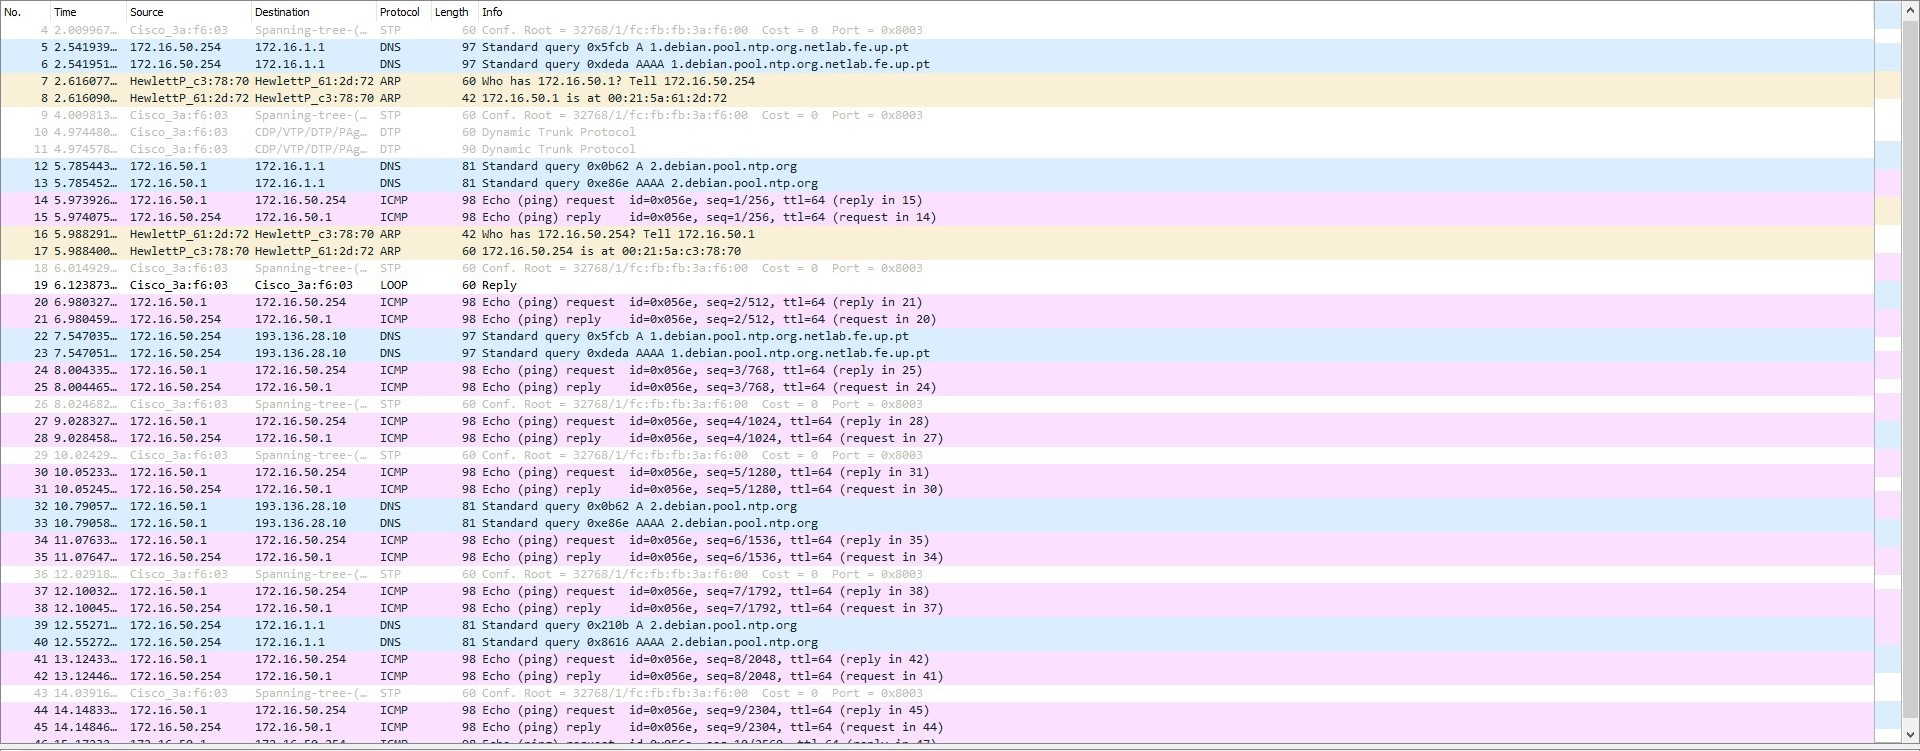
\includegraphics[width=\linewidth]{img/exp1.jpg}
  \caption{Experiência 1 - Resultado do ping de tux3 para tux4}
\end{figure}


\subsection{Experiência 2}

\begin{figure}[H]
\centering
  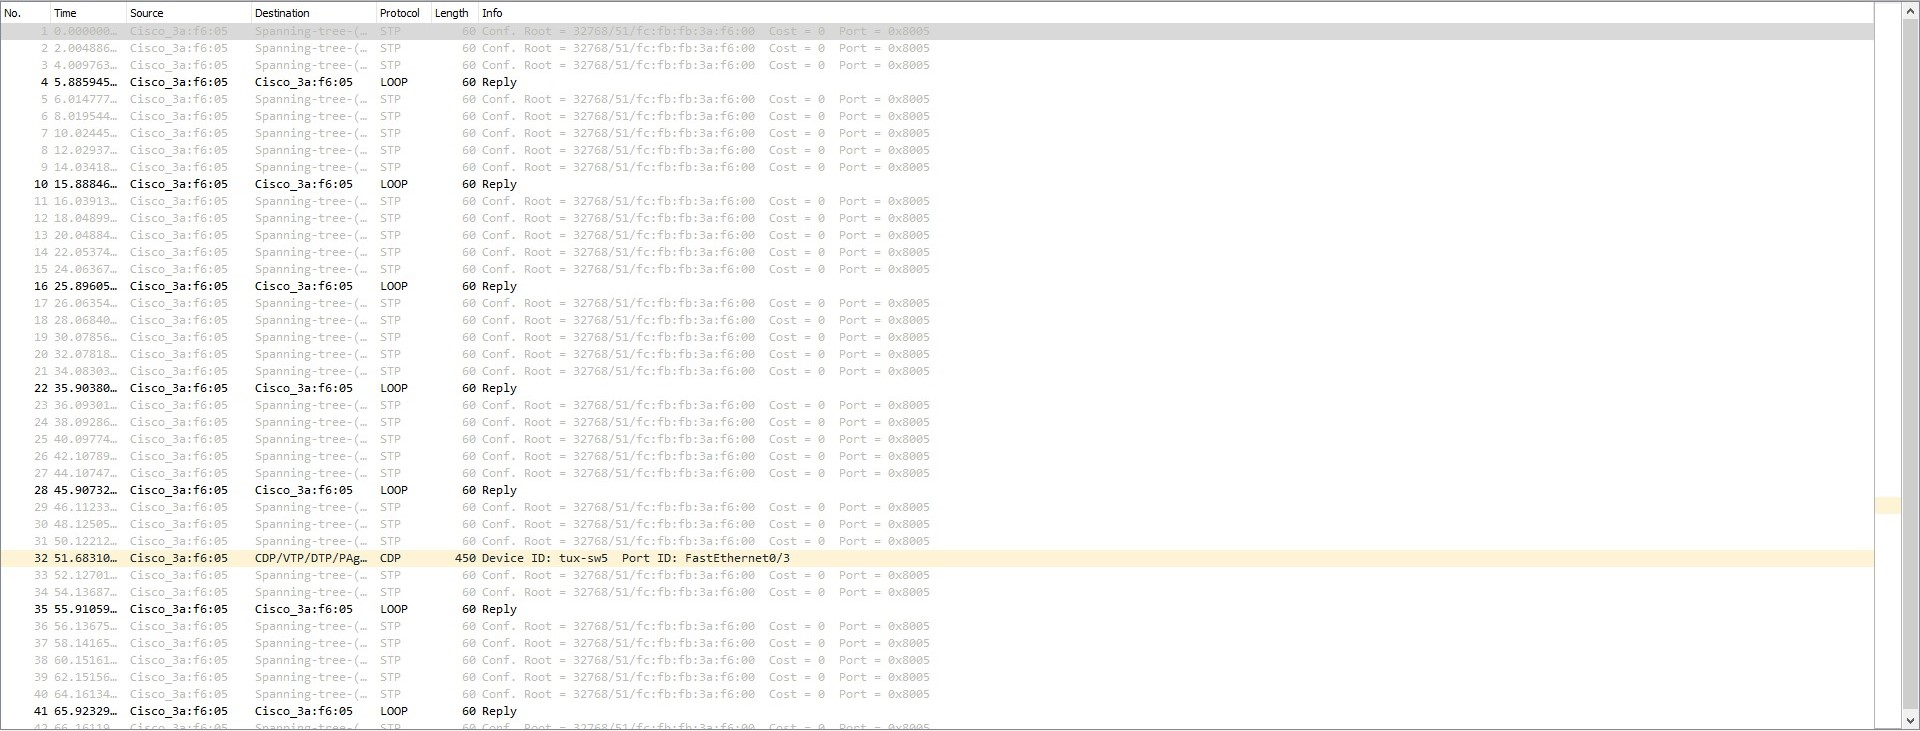
\includegraphics[width=\linewidth]{img/exp2-tsk8-tux2-full.jpg}
  \caption{Experiência 2 - Resultado do ping broadcast de tux3 em tux2}
\end{figure}

\begin{figure}[H]
\centering
  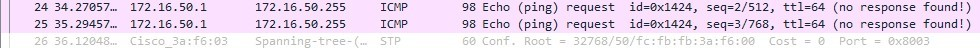
\includegraphics[width=\linewidth]{img/exp2-tsk8-tux3.jpg}
  \caption{Experiência 2 - tux3 ping broadcast tux3}
\end{figure}

\begin{figure}[H]
\centering
  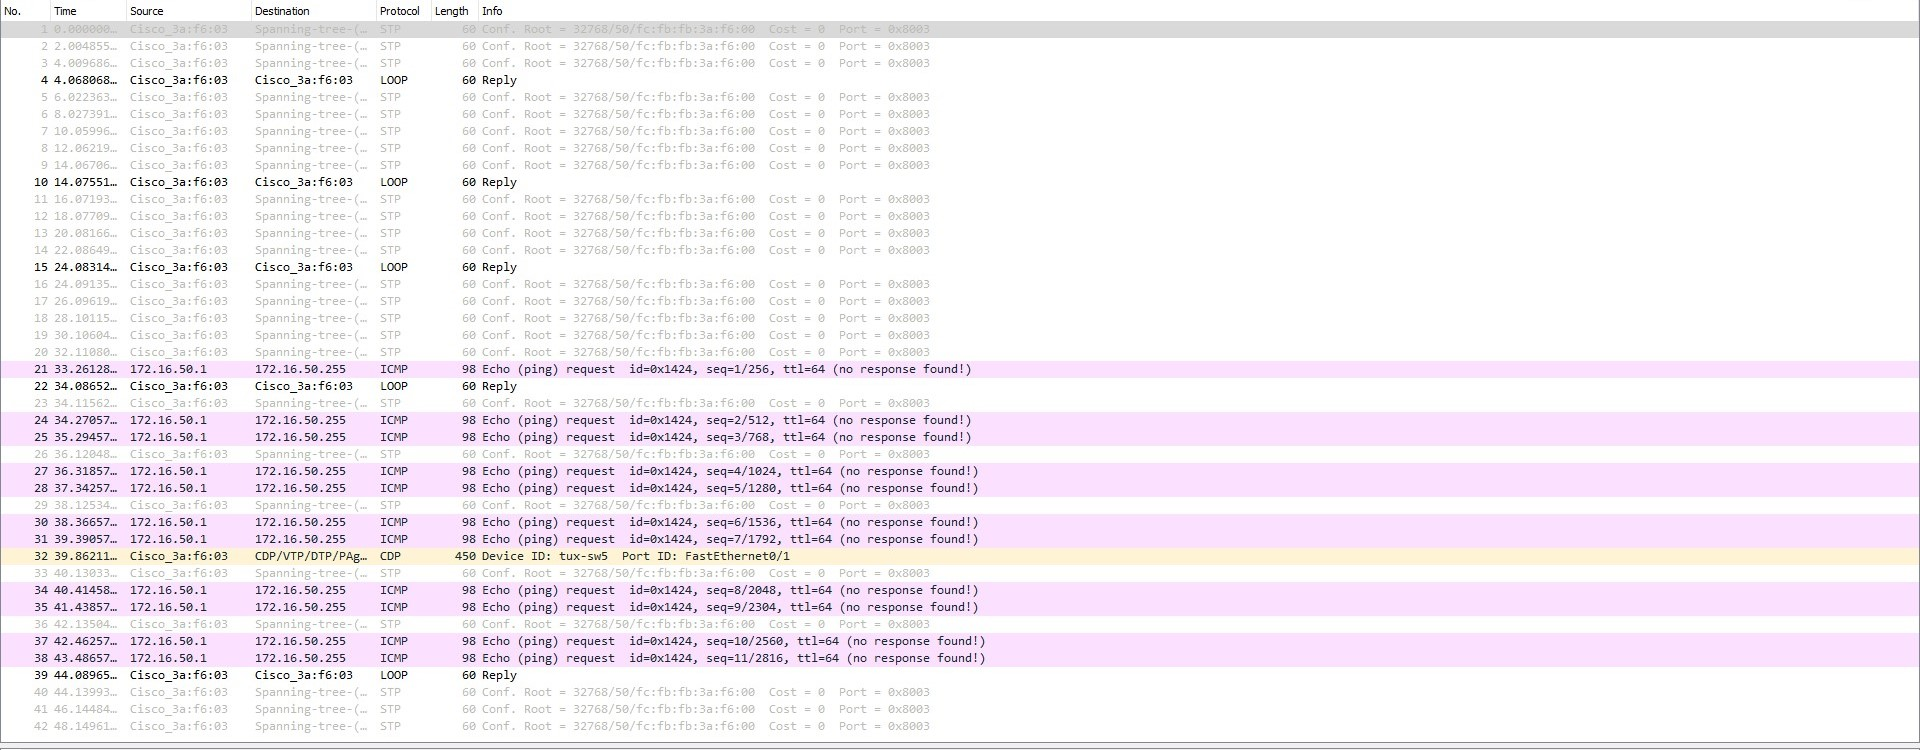
\includegraphics[width=\linewidth]{img/exp2-tsk8-tux3-full.jpg}
  \caption{Experiência 2 - Resultado do ping broadcast de tux3 em tux3}
\end{figure}

\begin{figure}[H]
\centering
  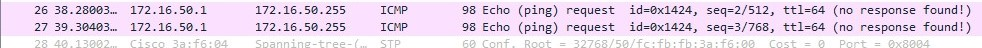
\includegraphics[width=\linewidth]{img/exp2-tsk8-tux4.jpg}
  \caption{Experiência 2 - tux3 ping broadcast tux4}
\end{figure}

\begin{figure}[H]
\centering
  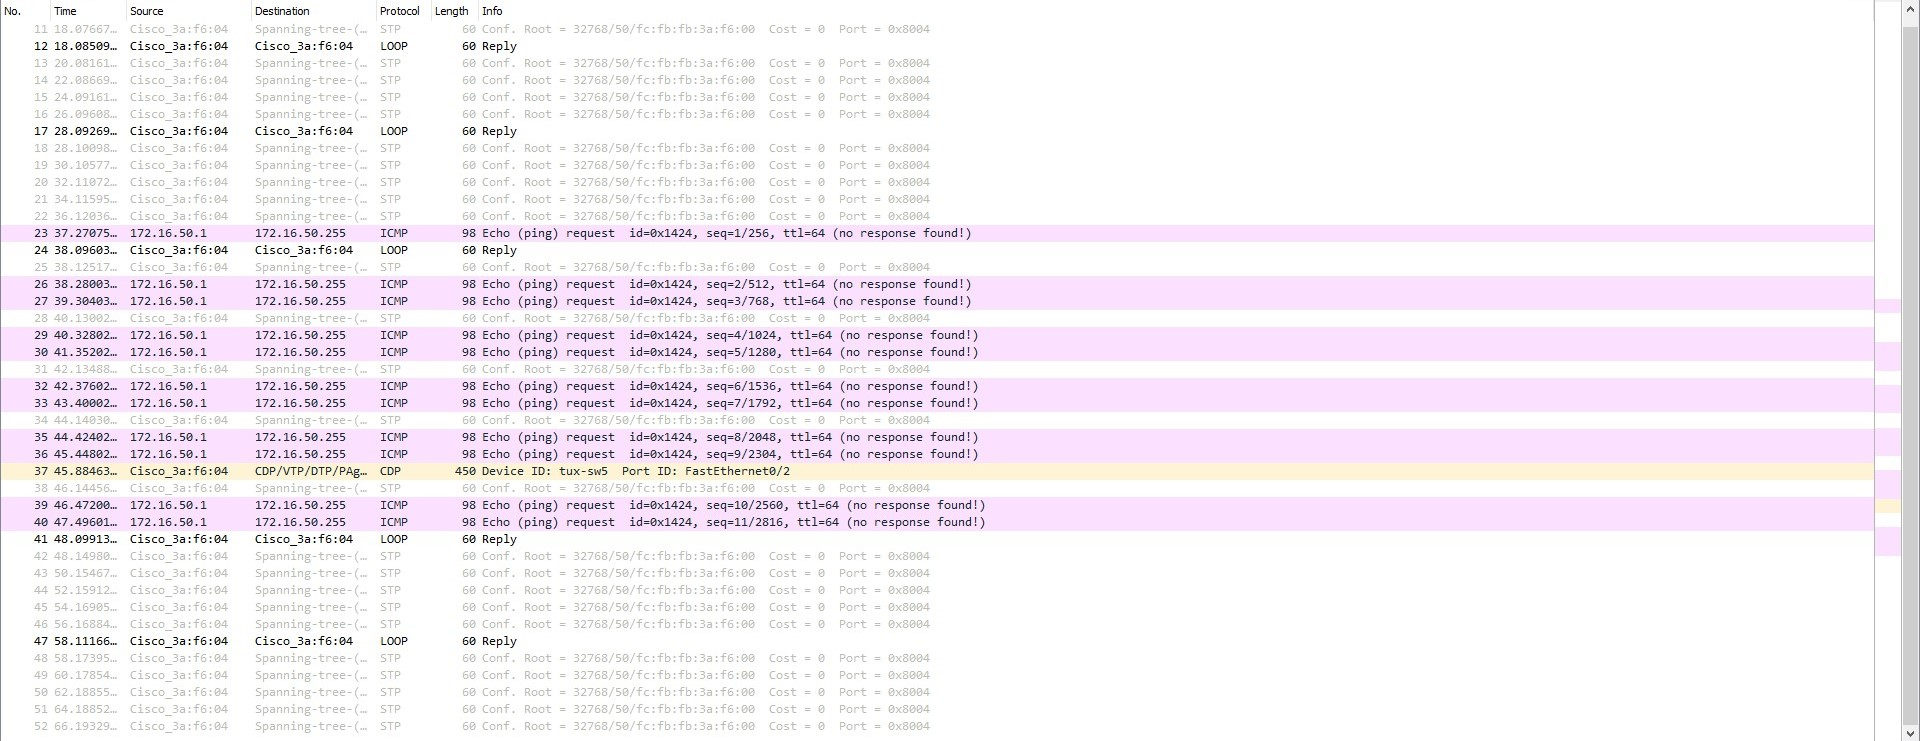
\includegraphics[width=\linewidth]{img/exp2-tsk8-tux4-full.jpg}
  \caption{Experiência 2 - Resultado do ping broadcast de tux3 em tux4}
\end{figure}

\begin{figure}[H]
\centering
  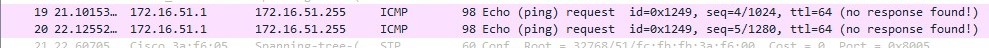
\includegraphics[width=\linewidth]{img/exp2-tsk10-tux2.jpg}
  \caption{Experiência 2 - tux2 ping broadcast}
\end{figure}

\begin{figure}[H]
\centering
  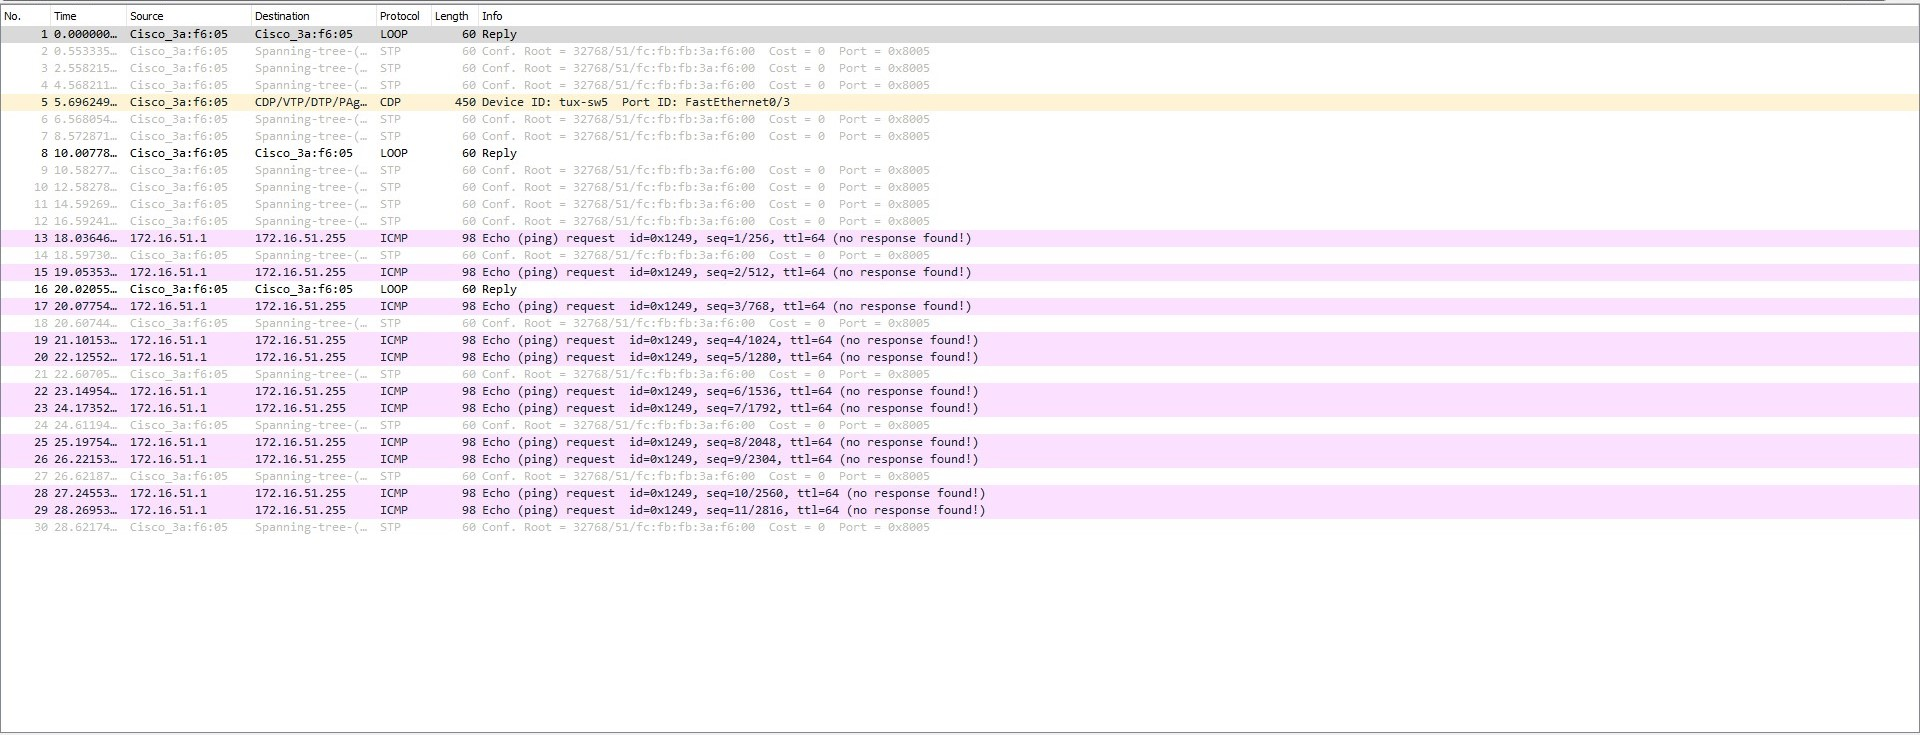
\includegraphics[width=\linewidth]{img/exp2-tsk10-tux2-full.jpg}
  \caption{Experiência 2 - Resultado do ping broadcast de tux2 em tux2}
\end{figure}

\begin{figure}[H]
\centering
  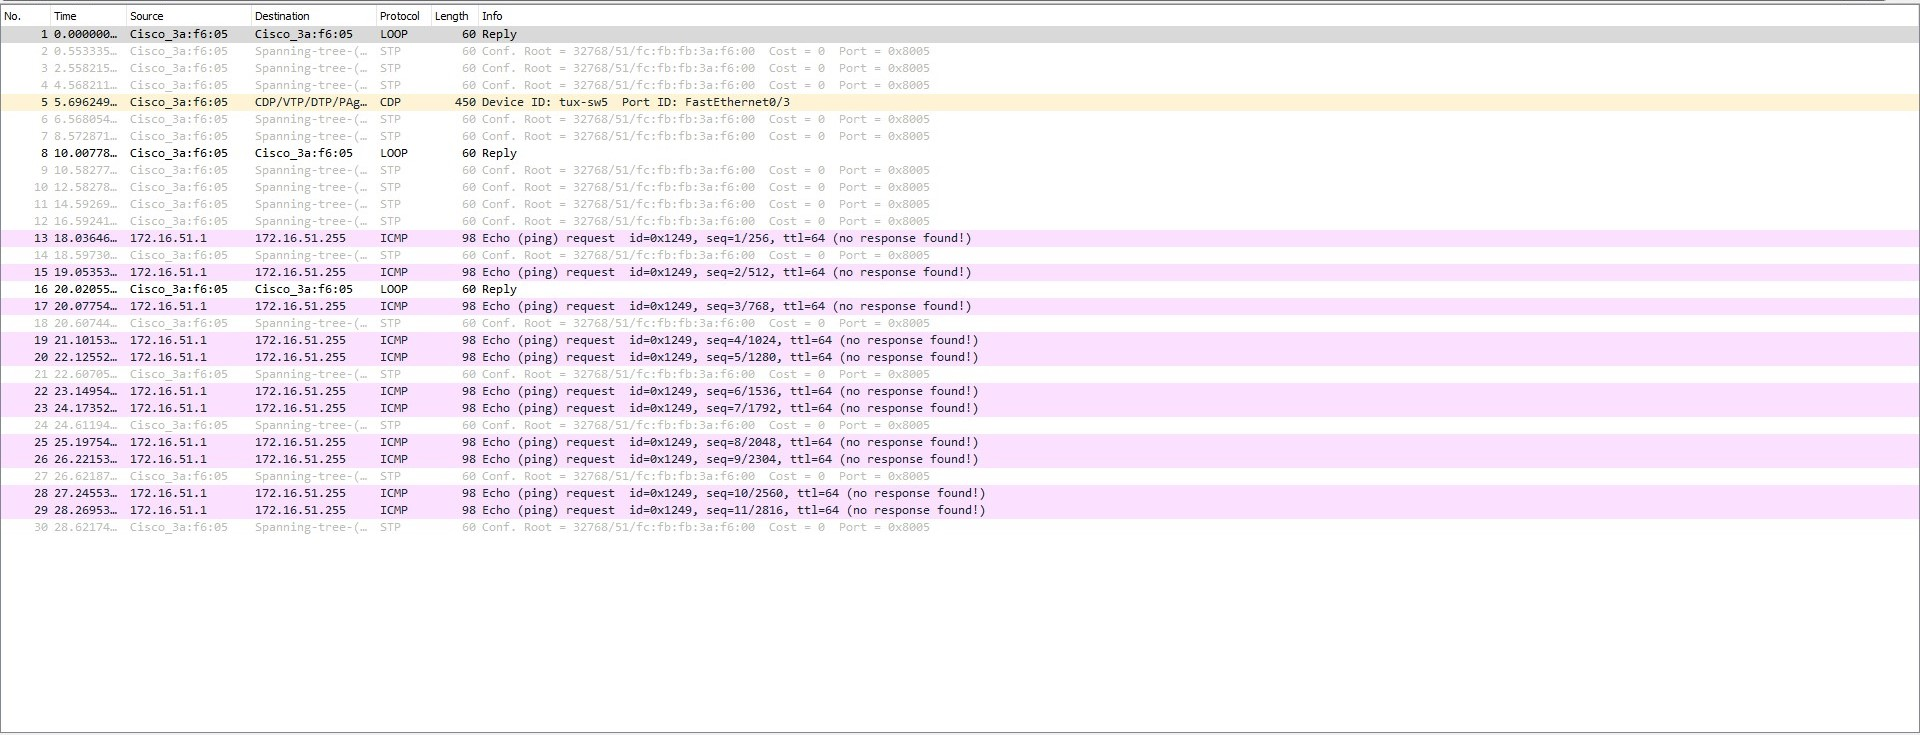
\includegraphics[width=\linewidth]{img/exp2-tsk10-tux2-full.jpg}
  \caption{Experiência 2 - Resultado do ping broadcast de tux2 em tux3}
\end{figure}

\begin{figure}[H]
\centering
  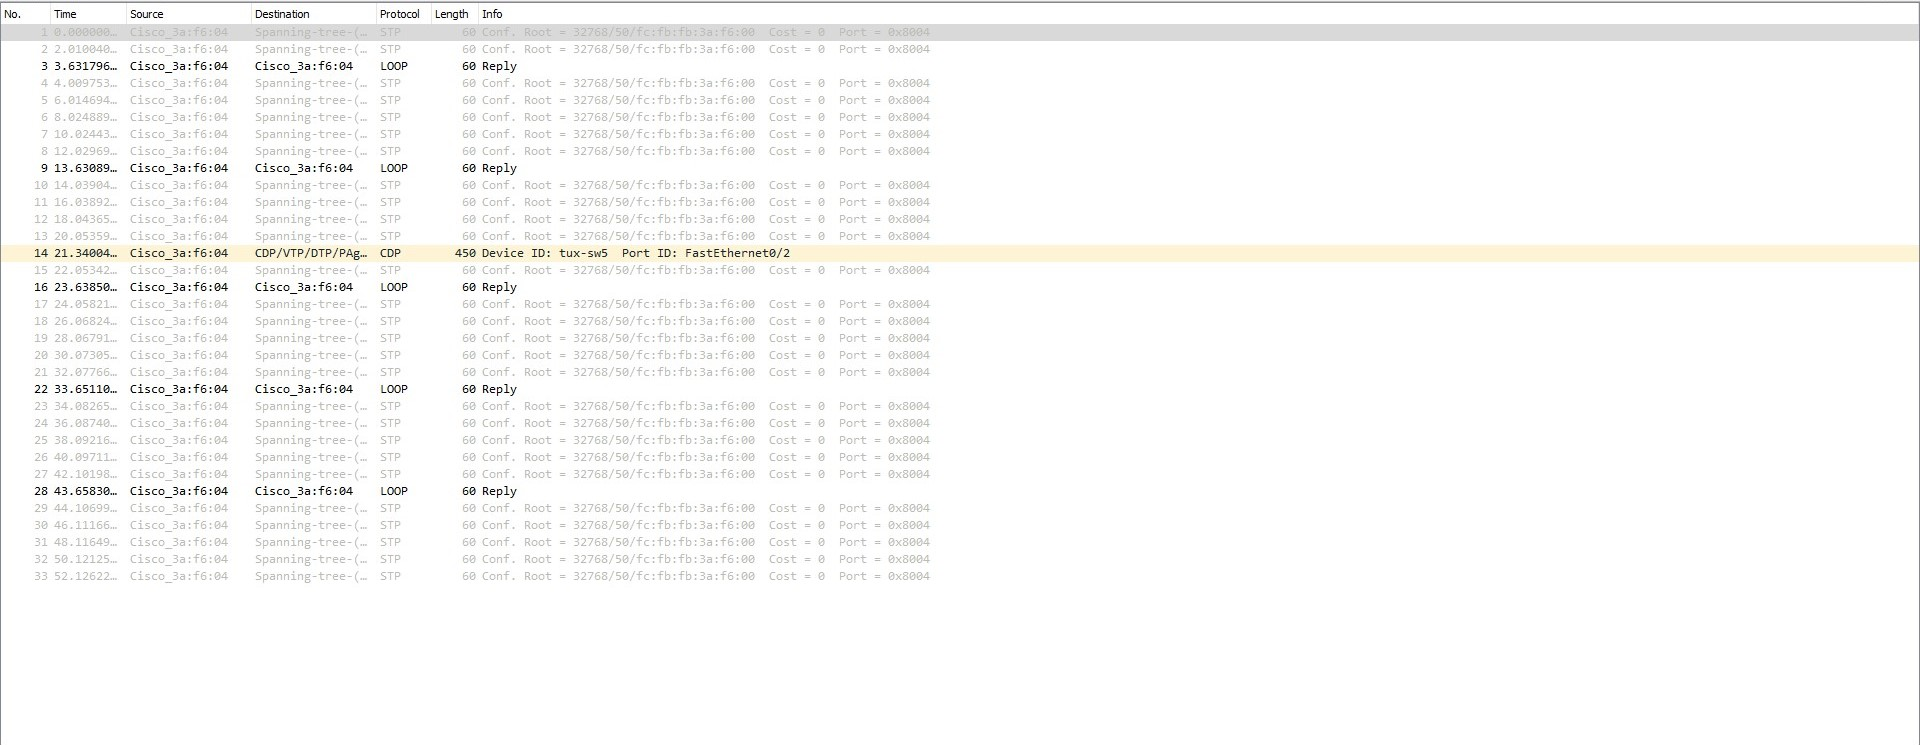
\includegraphics[width=\linewidth]{img/exp2-tsk10-tux4-full.jpg}
  \caption{Experiência 2 - Resultado do ping broadcast de tux2 em tux4}
\end{figure}


\subsection{Experiência 3}

\begin{figure}[H]
\centering
  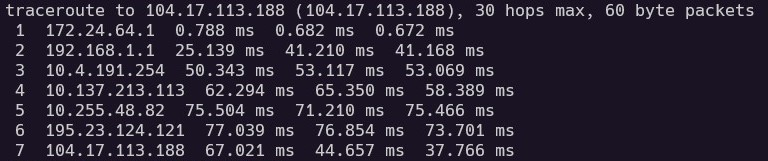
\includegraphics[width=\linewidth]{img/exp3-traceroute.jpg}
  \caption{Experiência 3 - Rota percorrida pelo pacote até atingir 104.17.113.188}
\end{figure}

\begin{figure}[H]
\centering
  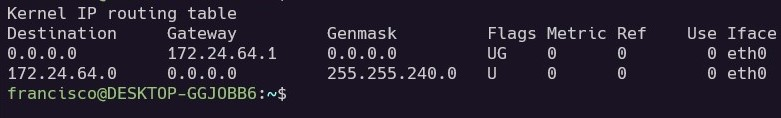
\includegraphics[width=\linewidth]{img/exp3-routes.jpg}
  \caption{Experiência 3 - Rotas presentes no computador}
\end{figure}

\begin{figure}[H]
\centering
  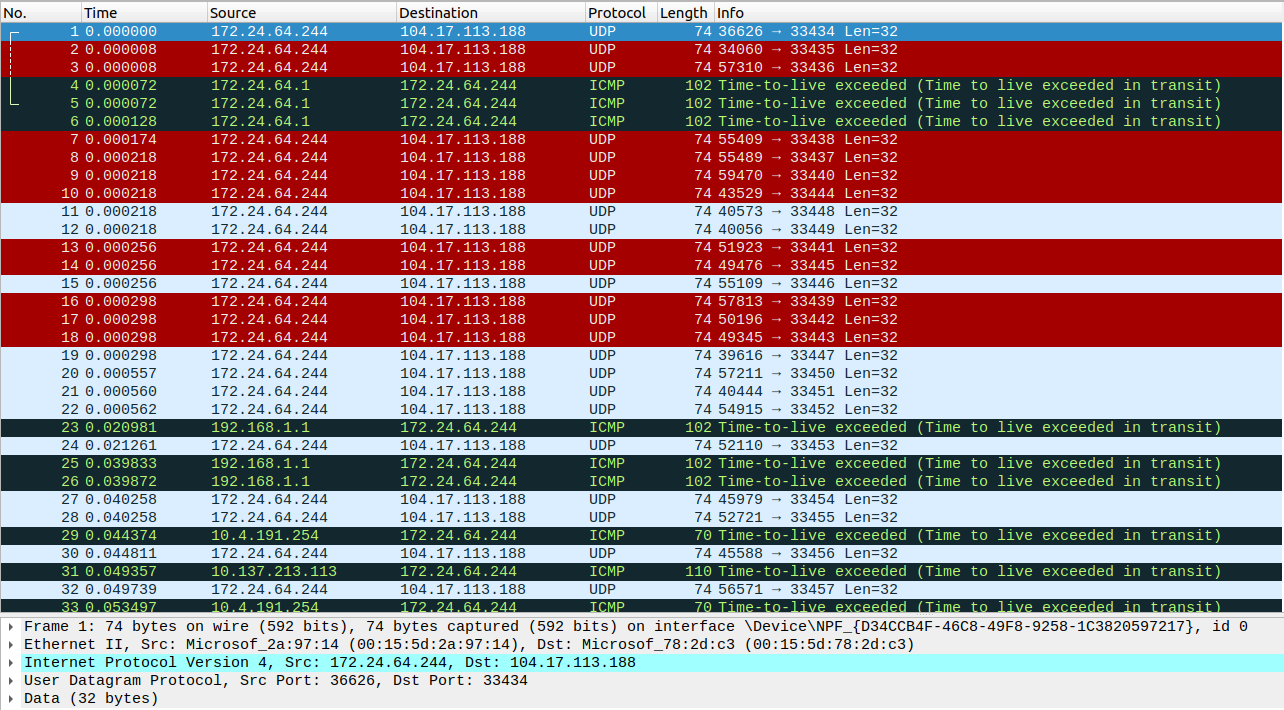
\includegraphics[width=\linewidth]{img/EXP3-traceroute.png}
  \caption{Experiência 3 - Resultado traceroute}
\end{figure}

\begin{figure}[H]
\centering
  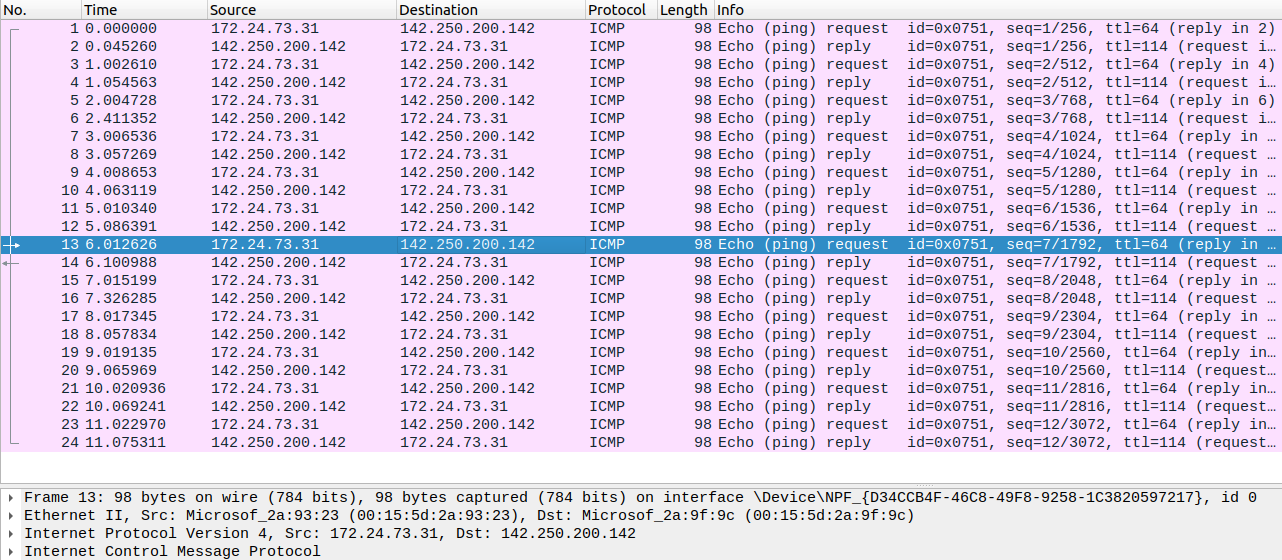
\includegraphics[width=\linewidth]{img/EXP3-youtubas.png}
  \caption{Experiência 3 - Resultado ping youtubas}
\end{figure}

\begin{figure}[H]
\centering
  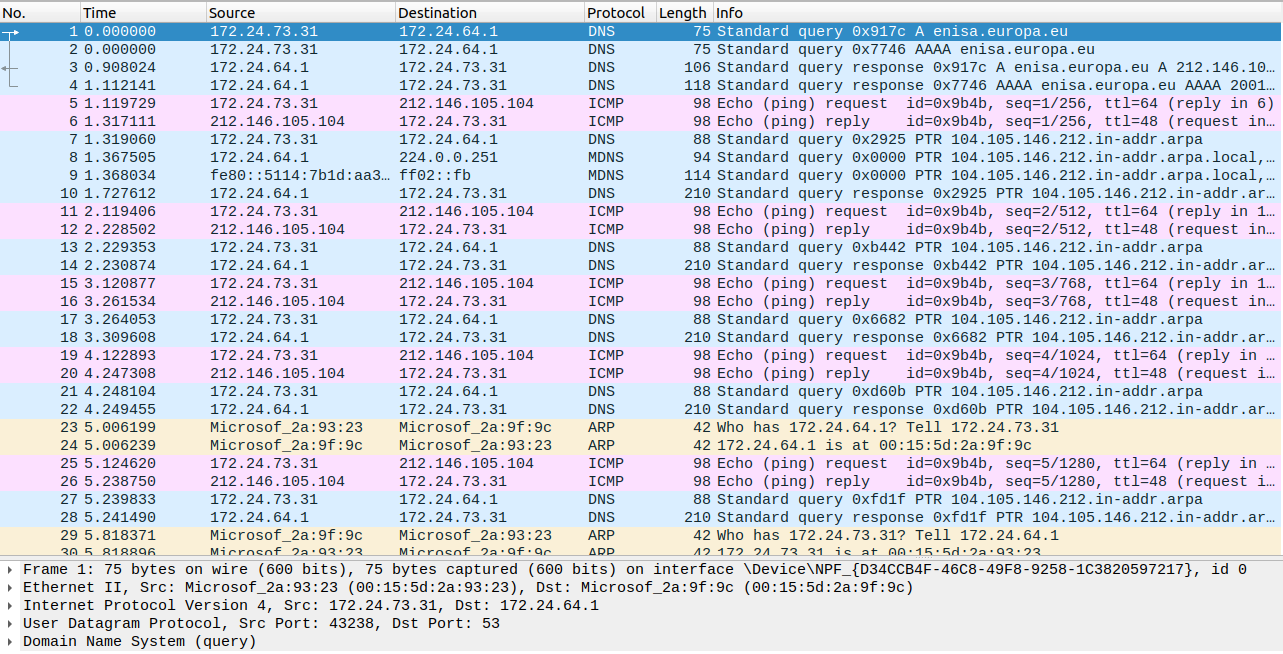
\includegraphics[width=\linewidth]{img/EXP3-enisa.png}
  \caption{Experiência 3 - Resultado ping enisa.europa.eu}
\end{figure}



\subsection{Experiência 4}

\begin{figure}[H]
\centering
  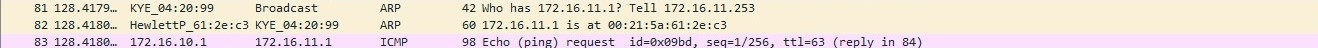
\includegraphics[width=\linewidth]{img/exp4-tux2-ask-tux4.jpg}
  \caption{Experiência 4 - tux4 pede MAC a tux2}
\end{figure}

\begin{figure}[H]
\centering
  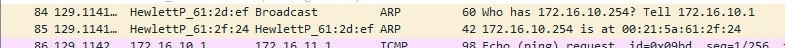
\includegraphics[width=\linewidth]{img/exp4-tux3-ask-tux4.jpg}
  \caption{Experiência 4 - tux3 pede MAC a tux4}
\end{figure}

\begin{figure}[H]
\centering
  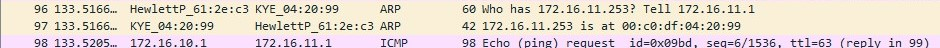
\includegraphics[width=\linewidth]{img/exp4-tux4-ask-tux2.jpg}
  \caption{Experiência 4 - tux2 pede MAC a tux4}
\end{figure}

\begin{figure}[H]
\centering
  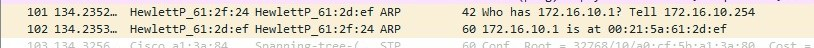
\includegraphics[width=\linewidth]{img/exp4-tux4-ask-tux3.jpg}
  \caption{Experiência 4 - tux4 pede MAC a tux3}
\end{figure}

\begin{figure}[H]
\centering
  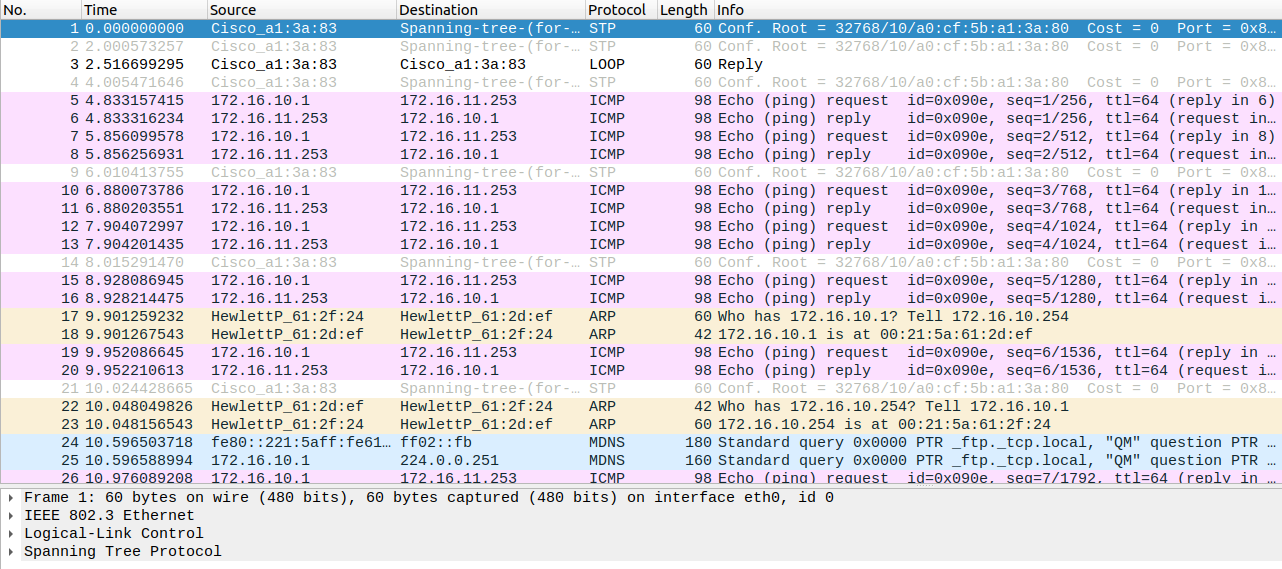
\includegraphics[width=\linewidth]{img/EXP4-3to4-253.png}
  \caption{Experiência 4 - Resultado de tux3 ping tux4 via 253}
\end{figure}

\begin{figure}[H]
\centering
  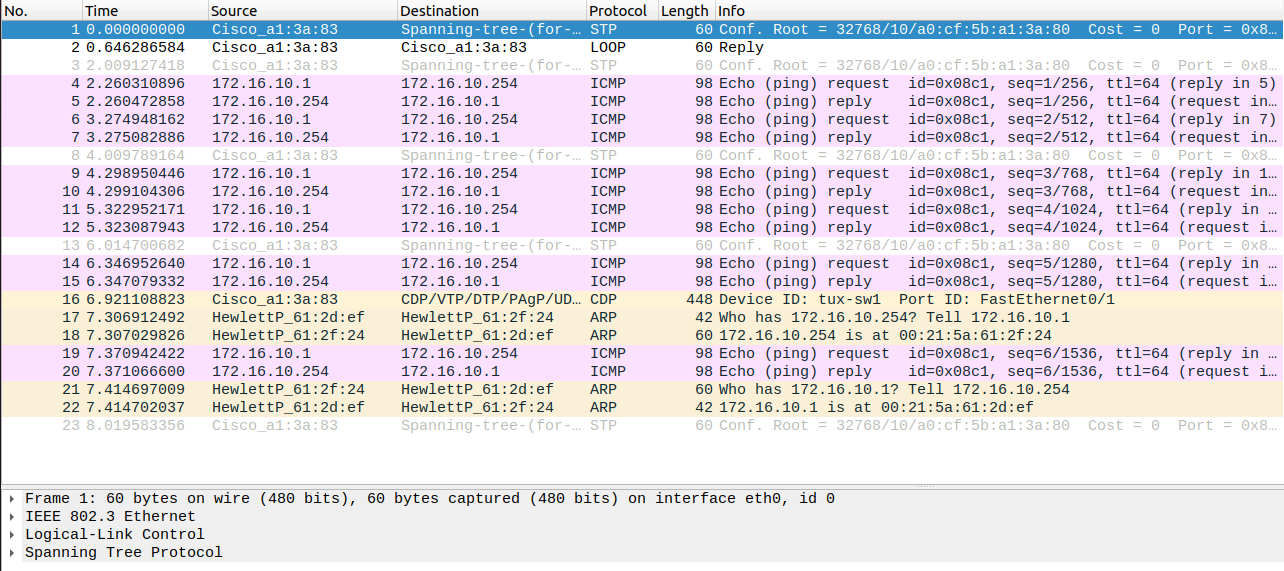
\includegraphics[width=\linewidth]{img/EXP4-3to4-254.png}
  \caption{Experiência 4 - Resulatdo de tux3 ping tux4 via 254}
\end{figure}

\begin{figure}[H]
\centering
  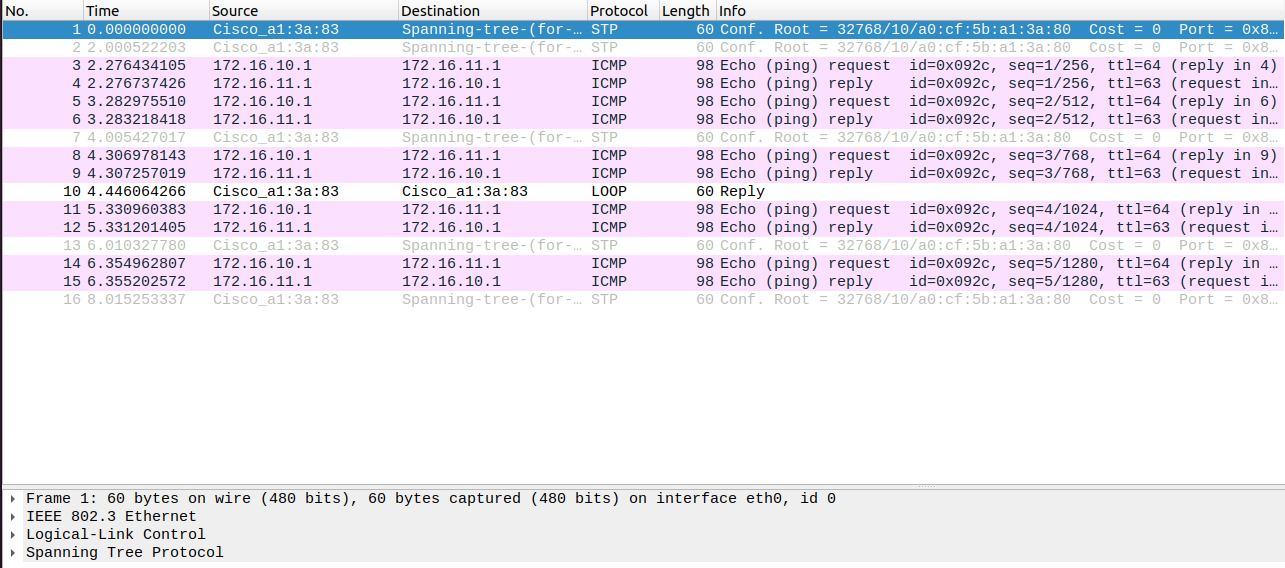
\includegraphics[width=\linewidth]{img/EXP4-3to2.png}
  \caption{Experiência 4 - Resultado de tux3 ping tux2}
\end{figure}

\begin{figure}[H]
\centering
  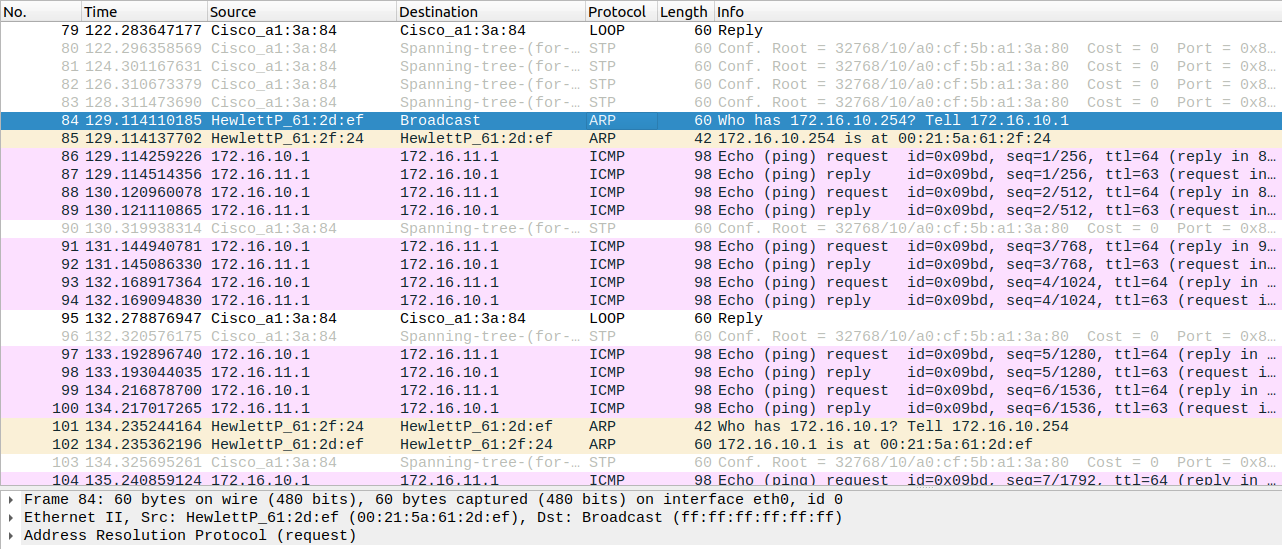
\includegraphics[width=\linewidth]{img/EXP4-task13-eth0.png}
  \caption{Experiência 4 - Resultado em tux4 eth0 de tux3 ping tux2}
\end{figure}

\begin{figure}[H]
\centering
  \includegraphics[width=\linewidth]{img/EXP4-task13-eth1.png}
  \caption{Experiência 4 - Resultado em tux4 eth1 de tux3 ping tux2}
\end{figure}




\end{document}